\documentclass[btech,thesis,twoside]{iist}
\usepackage{times} % Or your specific thesis class
\usepackage{amsmath}
\usepackage{amsfonts} % For mathbb if needed
\usepackage{amssymb}  % For math symbols
\usepackage{bm}       % For bold math symbols if preferred (e.g., \bm{A})
% \usepackage{amsmath} % Already included by iist.cls
% \usepackage{amsfonts} % Already included by amssymb loaded by iist.cls
% \usepackage{amssymb} % Already included by iist.cls
% \usepackage{bm} % Already included by iist.cls
\usepackage{graphicx} % Added for potential figure reference
\usepackage{algorithm}
\usepackage{algorithmicx}
% \usepackage{amsmath} % Already included
% \usepackage{amssymb} % Already included
% \usepackage{graphicx} % Already included
\usepackage{booktabs} % For professional-looking tables (optional, but recommended)
\usepackage{multirow} % For tables with multi-row cells (optional)
% \usepackage{subcaption} % Already included by iist.cls
\usepackage{algpseudocode}
% Add hyperref if you want clickable refs to equations/sections
\usepackage{hyperref} % Already present
% Add TikZ packages
\usepackage{tikz}
\usetikzlibrary{arrows.meta, backgrounds, fit, positioning, shapes.geometric} % Corrected to 'backgrounds'

% Add hyperref if you want clickable refs
% \usepackage{hyperref} % Already present
% \hypersetup{colorlinks=true, linkcolor=blue, citecolor=green, urlcolor=cyan} % Already present
\newcommand{\trainplotbase}{v1/project/MAPF-GNN-ADC/results/paper_plots}
% Define figure/table reference commands if needed
\newcommand{\reffig}[1]{Figure~\ref{#1}}
\newcommand{\reftab}[1]{Table~\ref{#1}}
\newcommand{\refsec}[1]{Section~\ref{#1}}
\hypersetup{colorlinks=true, linkcolor=blue, citecolor=green, urlcolor=blue} % Already present
\title{Decentralized Multi-Agent Path Planning }
\author{Velamala Rahul}
\studentid{SC21B127}
\advisor{Dr.Sourav Bhowmick}
\specialization{Electronics and Communication Engineering (Avionics)}
\department{Avionics}
\date{May 2025}


%% ---- Document starts here ---- %%

% ... rest of the document


%% ---- Document starts here ---- %%
\begin{document}

%% ---- Make the initial set of pages ---- %%
\maketitle % Title page
\makecertificate % Certificate 
\makedeclaration % Declaration
 % Dedication
\makeacknowledgements % Acknowledgements
\makeabstract % Abstract
\maketableofcontents % Table of contents
\makelistoffigures % List of figures
% \makelistoftables % List of tables
%\makelistofalgorithms % List of algorithms
\makeabbreviations % List of abbreviations
% \makenomenclature % Nomenclature (for symbols used)

% Initialize chapter settings; DO NOT comment this line
\makechaptersettings 


%% ---- Start chapters here ---- %%
\input{chapter1}
\chapter{Literature Review}
\label{chap:literature_review}
\section{Overview of Decentralized Multi-Agent Path Planning}
This chapter presents a comprehensive review of the methods and frameworks used in modern multi-agent path planning (MAPF) systems, especially those based on decentralized architectures.
It investigates various approaches to path planning in multi-robot systems, highlights the evolution towards decentralized and dynamically adaptive strategies, and discusses the increasing relevance of decentralized MAPF in complex and uncertain environments. Each section explores key concepts, technological advancements, and inherent challenges in developing and implementing decentralized MAPF solutions. The chapter aims to outline the state of the art, identify existing research gaps, and position the contributions of this work within the broader field.

\section{Multi-Agent Path Planning System Architectures}
A multi-agent path planning system can be broadly categorized based on its architecture, which dictates information flow and decision-making processes:
\begin{itemize}
    \item \textbf{Centralized Architectures:} In centralized systems, a single planning unit possesses complete knowledge of all agents, their goals, and the environment. This unit computes paths for all agents, ensuring coordination and often aiming for global optimality. Algorithms such as M* and CBS are key examples of this approach.
    \item \textbf{Decentralized Architectures:} Decentralized systems distribute planning and decision-making among individual agents. Each agent plans its path based on local information and limited communication with neighbors. Methods like VO and ORCA are representative of decentralized strategies.
    \item \textbf{Coupled Approaches:} Coupled approaches, often found in centralized systems, consider the joint state space of all agents simultaneously. This allows for optimal solutions but suffers from scalability issues. CBS and M* are examples of coupled approaches.
    \item \textbf{Decoupled Approaches:} Decoupled approaches simplify planning by considering each agent's path individually, addressing conflicts reactively. VO and ORCA are examples of decoupled methods that prioritize computational efficiency.
    \item \textbf{Networked Topologies:} Multi-agent systems often operate within networked topologies, where communication and coordination are constrained by the network structure. Graph-based representations, like those used in GNNs and algorithms like PRIMAL, are well-suited to model and exploit these topologies for decentralized MAPF.
\end{itemize}

\section{Centralized Multi-Agent Path Planning Techniques}
Centralized MAPF approaches, while offering optimality guarantees under certain conditions, face scalability limitations and single points of failure. This section reviews key centralized techniques and their characteristics.

\subsection{Optimal Centralized Algorithms: M* and ICTS}
Optimal centralized algorithms like M* \cite{Standley2011Complete}
and ICTS (Increasing Cost Tree Search) aim to find solutions with the minimum total cost (e.g., sum of path lengths) for all agents. M* guarantees optimality and completeness by systematically exploring the joint state space of all agents. ICTS, while also striving for optimality, improves efficiency over basic search algorithms by focusing on conflict resolution within a tree-based search framework. However, the computational complexity of these algorithms grows exponentially with the number of agents and environment size, limiting their applicability to large-scale problems.

\subsection{Conflict-Based Search (CBS)}
Conflict-Based Search (CBS) \cite{Sharon2015CBS}
is a prominent centralized MAPF algorithm that efficiently finds optimal or near-optimal solutions by iteratively resolving conflicts between agents paths. CBS operates on a two-level search structure: a high-level search that identifies and resolves conflicts by adding constraints, and a low-level search (typically A*) that replans paths for individual agents under these constraints. CBS significantly improves scalability compared to brute-force search methods but still faces computational challenges with increasing agent density and complex environments. Despite its efficiency improvements over purely exhaustive searches, CBS remains computationally expensive for very large teams or highly complex environments.

\section{Decentralized Multi-Agent Path Planning Techniques}
Decentralized MAPF methods prioritize scalability and robustness by distributing planning and decision-making among individual agents. This section reviews key decentralized approaches, including velocity obstacle based methods and learning-based techniques.

\subsection{Velocity Obstacle (VO) and Optimal Reciprocal Collision Avoidance (ORCA)}
Velocity Obstacle (VO) \cite{VanDenBerg2008ORCA}
and its refinement, Optimal Reciprocal Collision Avoidance (ORCA), are classic decentralized approaches for collision avoidance. VO defines a velocity obstacle for each agent based on the relative velocities and positions of neighboring agents. ORCA improves upon VO by ensuring reciprocal collision avoidance and smoother trajectories. These methods are computationally efficient and reactive, enabling real-time collision avoidance in dynamic environments. However, VO and ORCA are primarily reactive and may not guarantee goal achievement or optimality in complex scenarios, and can sometimes lead to local minima or deadlocks in tightly constrained spaces.

\subsection{Decentralized Planning with Graph Neural Networks (GNNs) and Adaptive Communication}
Recent advancements explore learning-based decentralized MAPF, particularly utilizing Graph Neural Networks (GNNs) and Reinforcement Learning (RL). GNNs, as demonstrated by Li et al. \cite{Li2021GNNCoordination},
are well-suited for decentralized MAPF due to their ability to model agent interactions within a graph structure, facilitating distributed information aggregation and decision-making. PRIMAL (Pathfinding via Reinforcement and Imitation Multi-Agent Learning) \cite{Sartoretti2019Primal} combines imitation learning from expert demonstrations with reinforcement learning to train decentralized policies, often without explicit communication modeling.

While GNNs show promise, standard approaches often rely on aggregating information from a \textbf{fixed K-hop neighborhood}. This means each agent communicates and integrates information only from peers within a predefined number of communication steps (hops). This fixed structure presents a limitation: the optimal communication range might vary depending on the environment density, the number of robots, or the specific tactical situation, and a single fixed K may not be universally optimal. Selecting the best K often requires manual tuning or heuristics, potentially limiting the adaptability and peak performance of the learned policy.

To address the limitations of fixed communication ranges, adaptive graph methods like Adaptive Diffusion Convolution (ADC) \cite{Zhao2021ADC} have been proposed in the broader GNN literature. ADC replaces discrete K-hop aggregation with a learnable diffusion process, characterized by a continuous radius parameter $t$. This parameter $t$, representing the effective extent of information propagation, is automatically learned during training, allowing the network itself to determine the most appropriate neighborhood size for feature aggregation based on the task objective. Integrating such adaptive diffusion mechanisms into GNNs for MAPF holds the potential to improve coordination policies by dynamically adjusting the communication neighborhood size, enhancing adaptability compared to fixed-K approaches.

\section{Relevance of Decentralized Multi-Agent Path Planning Systems}
Decentralized MAPF systems are increasingly relevant due to their inherent advantages in various robotic applications:
\begin{itemize}
    \item \textbf{Scalability:} Decentralized approaches scale more effectively to large teams of robots, as computational load is distributed across agents rather than concentrated in a central unit.
    \item \textbf{Robustness and Fault Tolerance:} Decentralized systems are more robust to failures, as the system can continue operating even if individual agents or communication links fail.
    \item \textbf{Adaptability to Dynamic Environments:} Decentralized agents can react more quickly to changes in the environment, as they rely on local sensing and communication rather than waiting for global updates.
    \item \textbf{Real-time Performance:} Decentralized algorithms are often more computationally efficient, enabling real-time path planning and execution, crucial for dynamic applications.
    \item \textbf{Versatility and Flexibility:} Decentralized systems can be deployed in diverse environments, including those with limited communication infrastructure or unknown topologies.
    \item \textbf{Cost-Effectiveness:} Decentralized systems can reduce reliance on expensive centralized computing and communication infrastructure, potentially lowering overall system costs.
    \item \textbf{Applications in Complex Domains:} Decentralized MAPF is essential for applications in domains like warehouse automation, autonomous driving, search and rescue, and space exploration, where large teams of robots must operate autonomously in dynamic and uncertain conditions.
\end{itemize}

\section{Challenges and Research Gaps in Decentralized MAPF}
\label{sec:challenges_gaps}
Despite their advantages, Decentralized MAPF systems face several significant challenges that represent active areas of research:
\begin{itemize}
    \item \textbf{Sub-optimality:} Decentralized solutions may not guarantee global optimality, as agents make decisions based on limited local information.
    \item \textbf{Deadlocks and Local Minima:} Insufficient coordination in decentralized systems can lead to deadlocks or agents becoming trapped in local minima.
    \item \textbf{Partial Observability:} Agents typically have only partial views of the environment, making it difficult to plan globally optimal paths and anticipate the actions of distant agents.
    \item \textbf{Communication Constraints and Strategy:}
        \begin{itemize}
            \item Limited communication range, bandwidth, or reliability can hinder effective coordination.
            \item \textbf{Gap:} Determining the optimal range and content of information to share remains a challenge. Specifically, most learning-based approaches, particularly GNNs, rely on \textit{fixed, predefined communication ranges (e.g., K-hops)}, which may not be suitable for diverse or dynamic scenarios. There is a need for mechanisms that allow the communication range to be learned or adapted.
        \end{itemize}
    \item \textbf{Dynamic and Uncertain Environments:} Adapting to dynamic obstacles, changing goals, and noisy sensor data in real-time remains a significant challenge.
    \item \textbf{Coordination Complexity:} Designing effective coordination mechanisms, especially for complex tasks and dense agent populations, is non-trivial.
    \item \textbf{Verification and Validation:} Verifying the correctness and safety of decentralized MAPF algorithms, particularly in safety-critical applications, can be challenging.
    \item \textbf{Adaptability and Learning in Decentralized Settings:}
        \begin{itemize}
            \item Enabling decentralized agents to learn robust policies that generalize well to unseen environments and tasks is an ongoing research area.
            \item \textbf{Gap:} While GNNs provide a framework for learning, their adaptability can be hampered by rigid structural assumptions, such as the aforementioned fixed communication ranges. Enhancing this adaptability is crucial.
        \end{itemize}
    \item \textbf{Balancing Reactivity and Proactiveness:} Decentralized agents need to be reactive to local changes while also exhibiting proactive behavior to achieve long-term goals and avoid potential future conflicts.
    \item \textbf{Ensuring Fairness and Efficiency:} In multi-agent systems, ensuring fairness in resource allocation and efficient overall system performance requires careful design of decentralized algorithms.
\end{itemize}

\subsection{Research Gaps Addressed by This Work}
\begin{enumerate}
    \item \textbf{Fixed Communication Range in GNN-based MAPF:} The primary gap tackled is the reliance of existing GNN-based decentralized MAPF frameworks (e.g., \cite{Li2021GNNCoordination}) on a fixed K-hop neighborhood for information aggregation. This work introduces an \textit{adaptive communication mechanism} by integrating Adaptive Diffusion Convolution (ADC) \cite{Zhao2021ADC}. This allows the effective communication range (diffusion radius $t$) to be learned automatically during training, rather than being manually predefined.
    \item \textbf{Limited Adaptability of Learned Policies:} By enabling the learning of an adaptive communication range, this work seeks to improve the adaptability of the learned coordination policies. The hypothesis is that allowing the network to determine the optimal extent of information propagation will lead to policies that perform more robustly across diverse environmental conditions (e.g., varying obstacle densities) and generalize better to unseen scenarios compared to models with fixed communication ranges.
\end{enumerate}
While there are still many challenges like finding the best possible solutions or dealing with fast-changing environments, this thesis mainly focuses on improving how robots communicate and adapt in learning-based decentralized MRPP.

\section{Chapter Summary}
This chapter has provided a literature review focusing on Decentralized Multi-Agent Path Planning. We explored the spectrum of MAPF approaches, from centralized optimal algorithms like M* and CBS to decentralized reactive methods like VO and ORCA, as well as emerging learning-based techniques utilizing GNNs, such as those by Li et al. \cite{Li2021GNNCoordination}, and RL-based methods like PRIMAL \cite{Sartoretti2019Primal}. A key challenge and research gap identified in current GNN-based learning methods is their reliance on fixed communication ranges, which can limit performance and adaptability across varied scenarios.

The chapter highlighted the relevance and advantages of decentralized MAPF in complex robotic applications, while also outlining the significant general challenges that remain. This thesis investigates the research gap concerning fixed communication ranges in GNN-based MAPF by exploring the use of Adaptive Diffusion Convolution (ADC) \cite{Zhao2021ADC} as a means to enable learning of effective and adaptive communication patterns. In the following chapters, we study how such adaptive communication mechanisms can influence the performance, robustness, and generalization capabilities of decentralized MAPF systems.
% ============================================================
% CHAPTER 3: BACKGROUND AND THEORETICAL FOUNDATIONS
% ============================================================
\chapter{Background and Theoretical Foundations}
\label{chap:background}

This chapter introduces the background needed to understand the proposed decentralized multi-robot path planning framework enhanced with Adaptive Diffusion Convolution (ADC). We begin by introducing fundamental concepts from graph theory, which provide the mathematical language for representing multi-robot systems and their interactions. We then delve into Graph Neural Networks (GNNs), explaining their general architecture and how they process graph-structured data, highlighting the limitations of standard fixed-neighborhood approaches. Subsequently, we explore concepts from graph signal processing and graph diffusion processes, focusing on the graph heat kernel, which forms the basis for ADC. Finally, we detail the Adaptive Diffusion Convolution mechanism itself, explaining how it enables learnable, adaptive information propagation on graphs, followed by a comparison of its theoretical properties against standard GCNs.

\section{Graph Theory Essentials}
\label{sec:graph_theory}

Graphs provide a natural and powerful way to model the relationships and interactions within multi-robot systems.

A \textbf{graph} is formally defined as a pair $G = (V, E)$, where $V$ is the set of vertices (or nodes) and $E \subseteq V \times V$ is the set of edges connecting pairs of vertices. In the context of MRPP, the set of robots typically constitutes the vertex set $V = \{1, ..., N\}$, where $N$ is the total number of robots.

An \textbf{edge} $(i, j) \in E$ signifies a relationship or potential interaction between robot $i$ and robot $j$. In decentralized MRPP, edges often represent the possibility of direct communication or sensing between robots. If the relationship is symmetric (i.e., if robot $i$ can communicate with $j$, then $j$ can communicate with $i$), the graph is \textbf{undirected}. If the relationship has a direction, the graph is \textbf{directed}. In many MRPP scenarios, communication links are bidirectional, leading to undirected graphs.

The structure of the graph, particularly the communication links, can change over time as robots move. Therefore, we often consider a \textbf{time-varying graph} $G_t = (V, E_t)$ at each discrete time step $t$. An edge $(i, j) \in E_t$ might exist if the distance between robots $i$ and $j$ at time $t$, denoted by $\|p_i(t) - p_j(t)\|$, is less than or equal to a predefined communication radius $r_{comm}$.

The structure of a graph $G_t$ at time $t$ is commonly represented using matrices:

\begin{itemize}
    \item \textbf{Adjacency Matrix ($A_t$):} An $N \times N$ matrix where $[A_t]_{ij} = 1$ if $(i, j) \in E_t$ and $i \neq j$, and $[A_t]_{ij} = 0$ otherwise. For undirected graphs, $A_t$ is symmetric ($A_t = A_t^T$). Often, self-loops are added, resulting in $\hat{A}_t = A_t + I$, where $I$ is the identity matrix. This allows a node to consider its own features during aggregation.
    \item \textbf{Degree Matrix ($D_t$):} An $N \times N$ diagonal matrix where the $i$-th diagonal element $[D_t]_{ii}$ represents the degree of node $i$, calculated as $[D_t]_{ii} = \sum_{j=1}^{N} [A_t]_{ij}$. It counts the number of edges connected to node $i$. If self-loops are included via $\hat{A}_t$, the corresponding degree matrix is $\hat{D}_t$, where $[\hat{D}_t]_{ii} = \sum_{j=1}^{N} [\hat{A}_t]_{ij}$.
\end{itemize}

These matrices are fundamental building blocks for defining operations on graph signals and for constructing GNN layers.

\section{Graph Shift Operators (GSOs)}
\label{sec:gsos}

A Graph Shift Operator (GSO) is an $N \times N$ matrix $S$ whose sparsity pattern reflects the underlying graph topology. That is, $[S]_{ij} \neq 0$ only if $i=j$ or $(j, i) \in E$ (or $(i,j) \in E$ depending on convention, but for symmetric operators derived from undirected graphs, it doesn't matter). GSOs represent linear, local operations on graph signals (features defined on the nodes). Applying a GSO $S$ to a matrix of node features $X \in \mathbb{R}^{N \times F}$ (where each row is a node's feature vector) results in $SX$, where the features at each node become a linear combination of features from its neighbors (as defined by the non-zero entries in $S$).

Common GSOs derived from the graph structure at time $t$ include:
\begin{itemize}
    \item \textbf{Adjacency Matrix ($A_t$ or $\hat{A}_t$):} Represents aggregation from direct neighbors (and self if $\hat{A}_t$ is used).
    \item \textbf{Graph Laplacian Matrices:} Laplacians capture notions of smoothness and variation of signals over the graph.
        \begin{itemize}
        
            \item \textbf{Symmetrically Normalized Adjacency Matrix ($\tilde{A}_t$):} Used prominently in GCNs, defined as $\tilde{A}_t = \hat{D}_t^{-1/2} \hat{A}_t \hat{D}_t^{-1/2}$ (equivalent to Eq. 1 in the concise paper, assuming $\hat{A}_t$ and $\hat{D}_t$). This normalization helps stabilize learning and accounts for varying node degrees.
            \item \textbf{Symmetrically Normalized Laplacian ($L_{norm, t}$):} Defined as $L_{norm, t} = I - \tilde{A}_t = I - \hat{D}_t^{-1/2} \hat{A}_t \hat{D}_t^{-1/2}$ (equivalent to Eq. 2). Its eigenvalues are bounded between 0 and 2, which is beneficial for analysis and stability.
        \end{itemize}
\end{itemize}
The choice of GSO fundamentally influences how information propagates within a GNN.

\section{Graph Neural Networks (GNNs)}
\label{sec:gnns}

Graph Neural Networks (GNNs) are a class of deep learning models designed to operate directly on graph-structured data. They leverage the graph topology to learn representations for nodes, edges, or entire graphs. The core idea behind most GNNs is the \textbf{message passing} paradigm \cite{Gilmer2017MessagePassing}, where nodes iteratively aggregate information from their local neighborhoods and update their own representations.

\subsection{General Framework}
A typical GNN layer $l$ performs the following steps for each node $i$:
\begin{enumerate}
    \item \textbf{Message Computation:} Each neighbor $j$ of node $i$ computes a message, often based on its own features $h_j^{(l-1)}$ and potentially the edge features $e_{ji}$.
    \item \textbf{Aggregation:} Node $i$ aggregates the incoming messages from its neighbors (defined by the graph structure, often using a permutation-invariant function like sum, mean, or max).
    \item \textbf{Update:} Node $i$ updates its hidden representation $h_i^{(l)}$ based on its previous representation $h_i^{(l-1)}$ and the aggregated message.
\end{enumerate}
Mathematically, many GNN layers can be expressed compactly using GSOs. Let $H^{(l)} \in \mathbb{R}^{N \times F^{(l)}}$ be the matrix of node features at layer $l$ (with $H^{(0)} = X$, the input features). A generic GNN layer can often be written as:
\begin{equation}
    H^{(l+1)} = \sigma \left( \text{AGGREGATE} \left( H^{(l)}, G_t \right) \cdot W^{(l)} \right)
\end{equation}
where $\sigma$ is a non-linear activation function (e.g., ReLU), $W^{(l)}$ is a learnable weight matrix for feature transformation, and $\text{AGGREGATE}(H^{(l)}, G_t)$ represents the neighborhood aggregation operation dictated by the graph $G_t$ (often involving a GSO).

\subsection{Graph Convolutional Network (GCN)}
The Graph Convolutional Network (GCN) \cite{Kipf2017GCN} is a popular and foundational GNN architecture. Its layer-wise propagation rule is:
\begin{equation}
    H^{(l+1)} = \sigma \left( \tilde{A}_t H^{(l)} W^{(l)} \right)
    \label{eq:gcn_layer}
\end{equation}
Here, the aggregation step is performed by multiplying with the symmetrically normalized adjacency matrix with self-loops, $\tilde{A}_t$. This effectively computes a weighted average of the features of a node and its immediate neighbors (1-hop neighborhood).

\subsection{Fixed Neighborhood Limitation}
A key characteristic of standard GCN layers (Eq. \ref{eq:gcn_layer}) is that they only aggregate information from the immediate 1-hop neighborhood in a single step. To capture information from nodes further away (K-hops), one typically needs to stack $K$ GCN layers. Alternatively, some architectures use graph polynomial filters \cite{Defferrard2016ChebNet}, where a single layer aggregates information over K-hops using powers of the GSO 
\begin{equation}
    H_{GNN} = f_{GNN}(X_t, S_t; K, \theta_{GNN}) = \sigma \left( \sum_{k=0}^{K-1} c_k S_t^k X_t W_k \right) \quad \text{(Conceptual form)}
\end{equation}
where $S_t$ is a GSO, $K$ defines the maximum hop count (filter degree), and $c_k, W_k$ are learnable parameters.

In both stacking layers and using polynomial filters, the extent of the neighborhood ($K$) is typically \textbf{fixed} and predefined. As discussed previously, this fixed nature is a major limitation in dynamic MRPP scenarios where the optimal communication range might vary.

\section{Graph Signal Processing and Diffusion Processes}
\label{sec:gsp_diffusion}

Graph Signal Processing (GSP) extends classical signal processing concepts to data defined on graph structures. It provides tools to analyze graph signals (features on nodes) in terms of their variation and smoothness with respect to the underlying graph topology.

\subsection{Graph Fourier Transform}
The eigendecomposition of a graph Laplacian matrix (e.g., $L_{norm} = U \Lambda U^T$, where $U$ contains the eigenvectors and $\Lambda$ is a diagonal matrix of eigenvalues) defines the Graph Fourier Transform (GFT). The eigenvectors $U$ form an orthonormal basis representing different modes of variation (graph frequencies), and the eigenvalues $\Lambda$ represent the corresponding frequencies. Small eigenvalues correspond to low frequencies (smooth signals over the graph), while large eigenvalues correspond to high frequencies (signals with rapid variations between neighbors).

\subsection{Diffusion Processes on Graphs}
Diffusion processes model the spread or flow of information (or heat, particles, etc.) over a network. A fundamental diffusion process on a graph, analogous to the heat equation in continuous space, can be described by the differential equation:
\begin{equation}
    \frac{dX(t)}{dt} = -L X(t)
    \label{eq:diffusion_pde}
\end{equation}
where $X(t) \in \mathbb{R}^{N \times F}$ represents the features/signal on the graph nodes at diffusion time $t$, and $L$ is a graph Laplacian operator.

\subsection{Graph Heat Kernel}
The solution to the diffusion equation (Eq. \ref{eq:diffusion_pde}) with an initial condition $X(0)$ is given by:
\begin{equation}
    X(t) = e^{-tL} X(0)
    \label{eq:diffusion_solution}
\end{equation}
The matrix exponential $H_t = e^{-tL}$ is known as the \textbf{graph heat kernel}. It acts as a linear operator that propagates the initial signal $X(0)$ over the graph structure for a diffusion time $t$.

Key properties of the heat kernel $H_t$:
\begin{itemize}
    \item \textbf{Low-pass Filter:} From a spectral perspective (using GFT), the heat kernel applies a filter $h(\lambda) = e^{-t\lambda}$ to the graph frequencies $\lambda$ (eigenvalues of $L$). Since $L$ is positive semi-definite ($\lambda \ge 0$), this filter attenuates high frequencies more strongly than low frequencies, effectively smoothing the signal over the graph.
    \item \textbf{Controlling Diffusion Extent:} The diffusion time parameter $t \ge 0$ controls the extent of smoothing and information propagation:
        \begin{itemize}
            \item As $t \to 0$, $H_t \to I$. There is no diffusion; each node retains only its initial information.
            \item As $t \to \infty$, $H_t$ projects the signal onto the graph's connected components' average values (assuming $L$ corresponds to a connected graph's Laplacian). Information spreads globally within components.
            \item For intermediate $t$, $H_t$ aggregates information from a neighborhood whose effective "radius" increases with $t$. This provides a principled way to control the scale of feature aggregation.
        \end{itemize}
\end{itemize}

\section{Adaptive Diffusion Convolution (ADC)}
\label{sec:adc}

The limitations of fixed-K GNNs motivate the use of more flexible aggregation mechanisms. Graph Diffusion Convolution (GDC) \cite{Klicpera2019DiffusionGCN} proposed using generalized diffusion processes (including PageRank and heat kernel) for feature propagation, but typically requires manual tuning of the diffusion parameters (like $t$ for the heat kernel) for each dataset.

Adaptive Diffusion Convolution (ADC) \cite{Zhao2021ADC} builds upon this by making the diffusion parameters \textbf{learnable}, allowing the network to automatically adapt the neighborhood size during training.

\subsection{ADC with Heat Kernel}
Focusing on the heat kernel, ADC employs $H_t = e^{-tL}$ as the feature propagation mechanism, where $L$ is typically chosen as $L = I - T$ with $T$ being a suitable GSO (e.g., $T=\tilde{A}_t$). The crucial difference is that the diffusion time $t$ is treated as a learnable parameter, optimized via backpropagation along with the network weights $W^{(l)}$.

\subsection{Implementation via Taylor Approximation}
Directly computing the matrix exponential $e^{-tL}$ is computationally expensive for large graphs. ADC relies on the Taylor series expansion. Since $L = I - T$, the heat kernel is $H_t = e^{-t(I-T)} = e^{-t} e^{tT}$. The term $e^{tT}$ can be approximated by truncating its Taylor series expansion:
\begin{equation}
    e^{tT} = \sum_{k=0}^{\infty} \frac{(tT)^k}{k!} \approx \sum_{k=0}^{K_{trunc}} \frac{t^k}{k!} T^k
\end{equation}
Combining these, the practical ADC propagation operator based on the truncated heat kernel becomes (similar to Eq. 10 in the concise paper):
\begin{equation}
    H_t \approx \sum_{k=0}^{K_{trunc}} \theta_k(t) T^k \quad \text{where} \quad \theta_k(t) = e^{-t} \frac{t^k}{k!}
    \label{eq:adc_approx_original} % Renamed to avoid conflict if needed elsewhere
\end{equation}
Here, $K_{trunc}$ is the truncation order (maximum hop distance considered in the approximation), and $T$ is the chosen GSO (e.g., $T = \tilde{A}_t$). The key is that the coefficients $\theta_k(t)$ depend on the \textit{learnable} parameter $t$. This allows the GNN layer using ADC:
\begin{equation}
    H^{(l+1)} = \sigma \left( \left( \sum_{k=0}^{K_{trunc}} \theta_k(t) T^k \right) H^{(l)} W^{(l)} \right)
\end{equation}
to adaptively control the influence of neighbors at different hop distances $k$ by learning the optimal diffusion time $t$.


% --- START OF REPLACEMENT ---
% \subsection{Theoretical Advantages}
% As highlighted in the concise paper (Sec VI) and \cite{Zhao2021ADC}:
% \begin{itemize}
%     \item \textbf{Stability:} If the chosen GSO $T$ satisfies $\|T\| \le 1$ (which $\tilde{A}_t$ does), the operator norm of the ADC propagation matrix (Eq. \ref{eq:adc_approx_original}) is bounded: $\|\sum_{k=0}^{K_{trunc}} \theta_k(t) T^k \| \le \sum_{k=0}^{K_{trunc}} |\theta_k(t)| \|T\|^k \le \sum_{k=0}^{\infty} \theta_k(t) = e^{-t}e^t = 1$. This inherent stability contrasts with standard GCN layers where the weights $W^{(l)}$ could potentially lead to exploding activations if not properly regularized.
%     \item \textbf{Adaptive Filtering:} Learning $t$ effectively means learning the cutoff frequency or bandwidth of the underlying low-pass heat kernel filter ($h(\lambda; t)=e^{-t\lambda}$). This allows the model to adapt the degree of signal smoothing based on the data and task, rather than using a fixed filter shape defined by K.
% \end{itemize}

% This ADC mechanism, particularly the learnable diffusion time $t$, forms the core of the adaptive communication module integrated into the MRPP framework proposed in this thesis (Chapter \ref{chap:methodology}). It replaces the fixed K-hop aggregation of standard GNNs, enabling more flexible and potentially more effective information sharing among robots.

% --- END OF REPLACEMENT ---

% --- START OF NEW SECTION ---
\section{Principal Technical Results}
\label{sec:principal_results}

This section provides a more detailed comparison of the theoretical properties, specifically stability and spectral filtering characteristics, between fixed-\(K\) Graph Neural Networks (like GCN) and the Adaptive Diffusion Convolution (ADC) approach utilized in this work.And these were the mathematical proof which shows why the ADC approach was chosen over the GCN approach.

\subsection{Stability Analysis}
We analyze the stability of the linear propagation operators inherent in GCN and ADC layers. Stability ensures that the magnitude of the node features does not grow uncontrollably through layers, which is crucial for reliable training and performance.
\newpage
\subsubsection{Notation and Assumptions for Analysis}
For the following analysis, let:
\begin{itemize}
    \item $\mathbf{S} \in \mathbb{R}^{N \times N}$ be a normalized graph shift operator (GSO), such as the symmetrically normalized adjacency matrix $\tilde{A}_t$ defined earlier, with spectral radius $\rho(\mathbf{S}) \le 1$. The spectral radius is the maximum absolute eigenvalue.
    \item $\mathbf{L} = \mathbf{I} - \mathbf{S}$ be the corresponding normalized Laplacian matrix. Its eigenvalues $\lambda_i$ satisfy $0 \le \lambda_i \le 2$. We can write its eigendecomposition as $\mathbf{L} = U \Lambda U^\top$, where $\Lambda = \mathrm{diag}(\lambda_1, \dots, \lambda_N)$.
    \item $\mathbf{T}$ be the propagation matrix used in ADC, assumed to satisfy $\|\mathbf{T}\| \le 1$. A common choice is $\mathbf{T} = \mathbf{S}$.
    \item $\|\cdot\|$ denote the induced $\ell_2$ operator norm (spectral norm). For symmetric matrices like $\mathbf{S}$ and $\mathbf{L}$, this is equal to the largest absolute eigenvalue.
\end{itemize}

\subsubsection{GCN Stability}
The linear part of a multi-hop GCN layer or a stack of GCN layers can often be represented as a polynomial filter applied to the node features:
\begin{equation}
P_{\mathrm{GCN}} = \sum_{k=0}^{K-1} \alpha_k \mathbf{S}^k
\label{eq:pgcn_poly}
\end{equation}
Here, $K$ represents the number of hops (or layers), $\mathbf{S}$ is the graph shift operator (GSO), and $\{\alpha_k\}$ are scalar coefficients effectively determined by the learned weight matrices $W^{(l)}$ across layers and any specific polynomial filter formulation (like ChebNet or the simplified GCN form). The stability of this operator is assessed by its operator norm, $\|P_{\mathrm{GCN}}\|$.

We can bound this norm as follows:
\begin{align}
    \|P_{\mathrm{GCN}}\| &= \left\| \sum_{k=0}^{K-1} \alpha_k \mathbf{S}^k \right\| && \text{(Definition from Eq. \ref{eq:pgcn_poly})} \nonumber \\
    &\le \sum_{k=0}^{K-1} \left\| \alpha_k \mathbf{S}^k \right\| && \text{(Triangle inequality for operator norms)} \nonumber \\
    &= \sum_{k=0}^{K-1} |\alpha_k| \left\| \mathbf{S}^k \right\| && \text{(Property of operator norms: } \|\beta \mathbf{X}\| = |\beta| \|\mathbf{X}\| \text{ for scalar } \beta \text{)} \label{eq:gcn_bound_step1}
\end{align}
Now, we consider the term $\|\mathbf{S}^k\|$. We use the submultiplicative property of operator norms, which states that $\|\mathbf{A}\mathbf{B}\| \le \|\mathbf{A}\|\|\mathbf{B}\|$. Applying this repeatedly:
\begin{equation}
    \|\mathbf{S}^k\| = \|\underbrace{\mathbf{S} \cdot \mathbf{S} \cdots \mathbf{S}}_{k \text{ times}}\| \le \underbrace{\|\mathbf{S}\| \cdot \|\mathbf{S}\| \cdots \|\mathbf{S}\|}_{k \text{ times}} = \|\mathbf{S}\|^k
    \label{eq:norm_sk_bound}
\end{equation}
In GCNs and many GNNs, the graph shift operator $\mathbf{S}$ (e.g., the symmetrically normalized adjacency matrix $\tilde{A}_t$) is typically normalized such that its spectral radius $\rho(\mathbf{S}) \le 1$. For symmetric matrices (like $\tilde{A}_t$), the operator norm (specifically, the 2-norm) is equal to its spectral radius, i.e., $\|\mathbf{S}\|_2 = \rho(\mathbf{S})$. Thus, if $\rho(\mathbf{S}) \le 1$, then $\|\mathbf{S}\| \le 1$. If $\mathbf{S}$ is not symmetric but is a normal matrix, the same holds. Even for general matrices, if we are considering the 2-norm, it's bounded by singular values, but the common normalization aims for $\rho(\mathbf{S}) \le 1$.

Assuming $\|\mathbf{S}\| \le 1$, then from Eq. \ref{eq:norm_sk_bound}:
\begin{equation}
    \|\mathbf{S}\|^k \le 1^k = 1
    \label{eq:norm_s_power_one}
\end{equation}
Therefore, $\|\mathbf{S}^k\| \le 1$.

Substituting this back into Eq. \ref{eq:gcn_bound_step1}:
\begin{equation}
    \|P_{\mathrm{GCN}}\| \le \sum_{k=0}^{K-1} |\alpha_k| (1) = \sum_{k=0}^{K-1} |\alpha_k|
    \label{eq:pgcn_final_bound}
\end{equation}
The last inequality (from the original text) holds because $\|\mathbf{S}^k\| \le \|\mathbf{S}\|^k \le 1^k = 1$ since $\mathbf{S}$ is typically normalized such that its spectral radius $\rho(\mathbf{S}) \le 1$ (implying $\|\mathbf{S}\| \le 1$ if $\mathbf{S}$ is symmetric or normal).

However, the crucial point is that the coefficients $\{\alpha_k\}$ are learned and generally \textit{unconstrained}. During training, the sum $\sum_{k=0}^{K-1} |\alpha_k|$ can potentially grow very large, leading to $\|P_{\mathrm{GCN}}\|$ exceeding 1 (as per the bound in Eq. \ref{eq:pgcn_final_bound}). This can cause exploding gradients or activations, making the network unstable without careful regularization or initialization strategies.
\subsubsection{ADC Stability}
ADC employs a propagation operator based on the truncated heat-kernel expansion, with coefficients determined by a \textit{learnable} diffusion time $t \ge 0$:
\begin{equation}
P_{\mathrm{ADC}}(t) = \sum_{k=0}^{K_{\mathrm{trunc}}} \theta_k(t)\,\mathbf{T}^k, \quad \text{where} \quad \theta_k(t) = e^{-t}\,\frac{t^k}{k!}
\end{equation}
Here, $K_{\mathrm{trunc}}$ is the truncation order of the Taylor series approximation for the heat kernel.

\begin{theorem}\label{thm:adc_stability}[ADC Stability Bound]
If the propagation matrix $\mathbf{T}$ satisfies $\|\mathbf{T}\| \le 1$, then for any diffusion time $t \ge 0$ and any truncation order $K_{\mathrm{trunc}} \ge 0$, the operator norm of the ADC propagation matrix is bounded by 1:
\begin{equation}
\|P_{\mathrm{ADC}}(t)\| \;\le\; 1.
\end{equation}
\end{theorem}

\begin{proof}
Using the triangle inequality and properties of the operator norm:
\begin{equation}
\|P_{\mathrm{ADC}}(t)\| = \left\|\sum_{k=0}^{K_{\mathrm{trunc}}}\theta_k(t)\,\mathbf{T}^k\right\| \;\le\; \sum_{k=0}^{K_{\mathrm{trunc}}}\left|\theta_k(t)\right|\,\|\mathbf{T}^k\|
\end{equation}
Since $t \ge 0$, the coefficients $\theta_k(t) = e^{-t} \frac{t^k}{k!}$ are non-negative, so $|\theta_k(t)| = \theta_k(t)$. Also, since $\|\mathbf{T}\| \le 1$, we have $\|\mathbf{T}^k\| \le \|\mathbf{T}\|^k \le 1^k = 1$. Therefore:
\begin{equation}
\|P_{\mathrm{ADC}}(t)\| \;\le\; \sum_{k=0}^{K_{\mathrm{trunc}}}\theta_k(t) \cdot 1 = \sum_{k=0}^{K_{\mathrm{trunc}}}\theta_k(t)
\end{equation}
This sum is a partial sum of the Taylor series for $e^t$, multiplied by $e^{-t}$. Since all terms are non-negative, the partial sum is less than or equal to the infinite sum:
\begin{equation}
\sum_{k=0}^{K_{\mathrm{trunc}}}\theta_k(t) \;\le\; \sum_{k=0}^{\infty}\theta_k(t) = \sum_{k=0}^{\infty} e^{-t}\,\frac{t^k}{k!} = e^{-t} \sum_{k=0}^{\infty} \frac{t^k}{k!} = e^{-t} e^{t} = 1
\end{equation}
Combining these steps, we get $\|P_{\mathrm{ADC}}(t)\| \le 1$.
\end{proof}

\noindent This result shows that the ADC aggregation mechanism is \textbf{inherently stable} due to the structure of the heat kernel coefficients. The operator norm is guaranteed to be bounded by 1, preventing the explosion of feature magnitudes regardless of the learned value of $t$ or the chosen truncation $K_{\rm trunc}$. This contrasts sharply with the potentially unbounded norm of the GCN operator.

\subsection{Spectral Filtering Characteristics}
We now analyze how GCN and ADC layers process graph signals in the frequency domain, defined by the eigenvalues $\lambda$ of the graph Laplacian $\mathbf{L}$. The behavior of a layer is characterized by its frequency response $h(\lambda)$.

\subsubsection{GCN as Polynomial Filter}
Consider the common GCN formulation using the normalized adjacency matrix $\mathbf{S} = \mathbf{I} - \mathbf{L}$. The propagation operator $P_{\mathrm{GCN}} = \sum_{k=0}^{K-1} c_k \mathbf{S}^k$ acts on the graph signal spectrum. Using the eigendecomposition $\mathbf{L} = U \Lambda U^\top$ (and thus $\mathbf{S} = U (\mathbf{I} - \Lambda) U^\top$), the spectral response of the GCN operator corresponding to an eigenvalue $\lambda$ of $\mathbf{L}$ is:
\begin{equation}
h_{\mathrm{GCN}}(\lambda) = \sum_{k=0}^{K-1} c_k (1 - \lambda)^k
\end{equation}
This shows that the GCN layer implements a graph filter whose frequency response is a \textbf{polynomial} in $(1-\lambda)$ of degree $K-1$. While the learnable coefficients $\{c_k\}$ offer flexibility in shaping the filter, the filter's complexity (degree) is \textbf{fixed} by the chosen number of hops/layers $K$. Selecting an appropriate $K$ is often crucial and problem-dependent.

\subsubsection{ADC as Exponential Filter}
The ideal (non-truncated) graph heat kernel is defined as the matrix exponential $\exp(-t\mathbf{L})$. Its spectral response can be found using the functional calculus on the Laplacian eigenvalues:
\begin{equation}
h_{\mathrm{ADC, ideal}}(\lambda; t) = e^{-t\lambda}
\end{equation}
The ADC layer, using the truncated approximation $P_{\mathrm{ADC}}(t) \approx \exp(-t(\mathbf{I}-\mathbf{T}))$, aims to approximate this behavior. The function $e^{-t\lambda}$ is a classic \textbf{low-pass filter}. For $\lambda=0$ (corresponding to the constant signal on connected components), the response is $e^0 = 1$. As the frequency $\lambda$ increases, the response decays exponentially.

\begin{theorem}\label{thm:adc_adaptivity}[ADC Filter Adaptivity]
The spectral response $h_{\mathrm{ADC, ideal}}(\lambda;t) = e^{-t\lambda}$ corresponds to a low-pass filter whose cutoff frequency and steepness are continuously controlled by the diffusion time parameter $t$. By learning $t$ through backpropagation, the ADC layer can adapt the filter's bandwidth (i.e., the degree of smoothing or the effective neighborhood size) to best suit the data and task.
\end{theorem}

\begin{proof}
Using the eigendecomposition $\mathbf{L}=U\Lambda U^\top$, the matrix exponential is $\exp(-t\mathbf{L}) = U\,\exp(-t\Lambda)\,U^\top$. The matrix $\exp(-t\Lambda)$ is diagonal with entries $e^{-t\lambda_i}$.
For a fixed $t > 0$:
\begin{itemize}
    \item If $\lambda_i$ is small (low frequency), $e^{-t\lambda_i}$ is close to 1, preserving the signal component.
    \item If $\lambda_i$ is large (high frequency), $e^{-t\lambda_i}$ is close to 0, attenuating the signal component.
\end{itemize}
The transition between passing and attenuating frequencies depends on $t$. As $t$ increases, the exponential decay becomes steeper, meaning the filter becomes more aggressively low-pass, suppressing higher frequencies more strongly and effectively averaging over larger neighborhoods. Conversely, as $t \to 0$, $e^{-t\lambda} \to 1$ for all $\lambda$, approaching an identity filter (no aggregation). Since $t$ is learned, the model can choose the optimal level of smoothing/aggregation.
\end{proof}

The truncated ADC operator $P_{\mathrm{ADC}}(t)$ provides a polynomial approximation to this ideal exponential filter, still retaining the adaptive control via the learnable $t$.

\subsection{Summary of Theoretical Advantages of ADC over Fixed-K GCN}
Based on the analysis above, ADC offers significant theoretical advantages:

\begin{enumerate}
    \item \textbf{Guaranteed Stability:} ADC's propagation operator norm is inherently bounded by 1 (Theorem \ref{thm:adc_stability}), preventing issues related to exploding feature norms without requiring explicit regularization on the propagation weights. GCN operators lack this guarantee as their norm depends on potentially unbounded learned coefficients. This inherent stability can lead to more robust training.
    \item \textbf{Adaptive Spectral Filtering:} ADC implements a graph filter based on the heat kernel $e^{-t\lambda}$, whose low-pass characteristics (bandwidth, neighborhood size) are continuously controlled by the \textit{learnable} parameter $t$ (Theorem \ref{thm:adc_adaptivity}). This allows the model to automatically adapt the extent of information aggregation based on the task and data distribution. GCN, in contrast, uses a polynomial filter whose degree (complexity) is fixed by the predetermined hyperparameter $K$, limiting its adaptability.
\end{enumerate}

These properties suggest that ADC can provide a more robust, stable, and adaptive mechanism for information propagation in GNNs compared to standard fixed-K GCN layers, potentially leading to better performance, especially in dynamic scenarios like MRPP where the optimal communication range might vary.


% --- END OF NEW SECTION ---


% End of Chapter 3
% Add bibliography command here in your main file: \bibliography{your_bib_file}
\input{chapter3}
\chapter{Framework \& Methodology}
\label{chap:methodology}

\section{Decentralized Framework Architecture}

The proposed decentralized multi-agent path planning framework is designed to enable each robot to make autonomous decisions based on local observations and communication with nearby agents. The overall architecture, illustrated in Figure~\ref{fig:framework_architecture}, comprises three main components: a Convolutional Neural Network (CNN) for local feature extraction from sensor data, an advanced Graph Neural Network (GNN) module based on Adaptive Diffusion Convolution (ADC) for inter-agent information aggregation and coordination, and a Multi-Layer Perceptron (MLP) that serves as an action policy network.

\begin{figure}[h]
    \centering
    \includegraphics[width=1\textwidth]{images/framework_figure.png} % Replace with your actual figure file and name
    \caption{General Decentralized Framework Architecture for Multi-Agent Path Planning, highlighting the flow from observation to action through CNN, GNN, and MLP components.}
    \label{fig:framework_architecture}
    \cite{Li2021GNNCoordination}
\end{figure}

The core innovation of this thesis lies in the GNN component, where a standard fixed-hop GNN is replaced by an Adaptive Diffusion Convolution (ADC) mechanism. This enhancement allows for more flexible and adaptive communication strategies among robots. Figure~\ref{fig:adc_enhanced_architecture_detail} provides a more detailed view of this ADC-enhanced framework, emphasizing the components of the adaptive communication module.
\begin{figure}
    \centering
    \includegraphics[width=0.7\textwidth]{images/block_diagram.png} % Replace with your actual figure file and name
    \caption{Detailed architecture of the ADC-enhanced MRPP framework.}
\label{fig:adc_enhanced_architecture_detail}
\end{figure}
\begin{comment}
\begin{figure}[t]
\centering
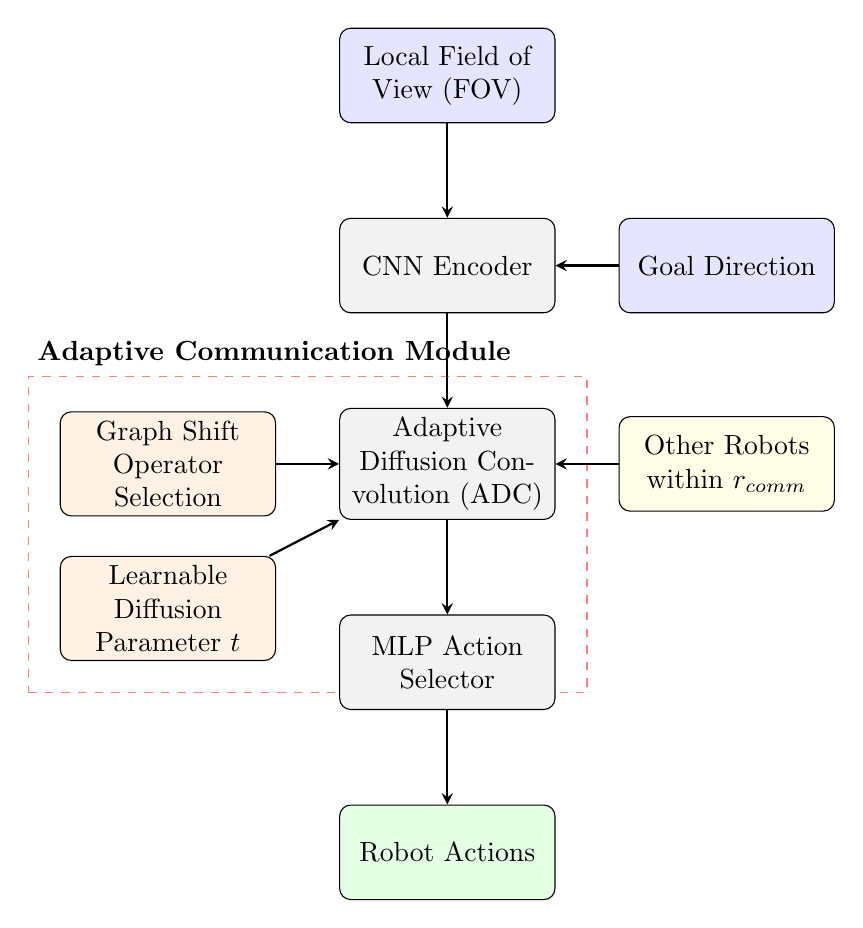
\begin{tikzpicture}[
    node distance=1.2cm,
    box/.style={rectangle, draw, minimum width=2.5cm, minimum height=1.2cm, text centered, rounded corners, text width=2.5cm},
    arrow/.style={thick,->,>=stealth},
    process/.style={rectangle, draw, fill=gray!10, minimum width=2.5cm, minimum height=1.2cm, text centered, rounded corners, text width=2.5cm},
    decision/.style={diamond, draw, fill=gray!10, minimum width=2.5cm, minimum height=1.2cm, text centered, text width=1.6cm}
]
% Nodes
\node[box, fill=blue!10] (fov) {Local Field of View (FOV)};
\node[process, below=of fov] (cnn) {CNN Encoder};
\node[process, below=of cnn] (gnn) {Adaptive Diffusion Convolution (ADC)};
\node[process, below=of gnn] (mlp) {MLP Action Selector};
\node[box, below=of mlp, fill=green!10] (action) {Robot Actions};
% Left side elements - Adjusted positioning to be closer
\node[box, left=0.8cm of gnn, fill=orange!10] (gsol) {Graph Shift Operator Selection};
\node[box, below=0.5cm of gsol, fill=orange!10] (diffusion) {Learnable Diffusion Parameter $t$};
% Right side elements - Adjusted positioning to be closer
\node[box, right=0.8cm of gnn, fill=yellow!10] (robots) {Other Robots within $r_{comm}$};
\node[box, right=0.8cm of cnn, fill=blue!10] (goal) {Goal Direction};
% Arrows
\draw[arrow] (fov) -- (cnn);
\draw[arrow] (goal) -- (cnn);
\draw[arrow] (cnn) -- (gnn);
\draw[arrow] (gnn) -- (mlp);
\draw[arrow] (mlp) -- (action);
\draw[arrow] (gsol) -- (gnn);
\draw[arrow] (diffusion) -- (gnn);
\draw[arrow] (robots) -- (gnn);
% Add a background container for the ADC part - Adjusted fit with label inside
\begin{scope}[on background layer]
\node[fit=(gsol) (diffusion) (gnn), draw=red!50, dashed, inner sep=0.4cm] (adc_box) {};
\end{scope}
% Place the label manually above the dashed box and to the left to avoid the arrow
\node[text=black, font=\bfseries, anchor=south west] at (adc_box.north west) {\textbf{Adaptive Communication Module}};
\end{tikzpicture}
\caption{Detailed architecture of the ADC-enhanced MRPP framework.}
\label{fig:adc_enhanced_architecture_detail}
\end{figure}
\end{comment}
\subsection{Observation Processing with Convolutional Neural Network}

Each robot is equipped with sensors that provide a local observation of its surroundings.The input is represented as a $W_{FOV} \times H_{FOV} \times 3$ tensor. This tensor, encompassing the local map, goal information (relative direction or position), and positions of other agents within the FOV, is processed by a CNN. The CNN acts as a feature extractor, designed to learn salient spatial features from this local observation, encoding information about obstacles, goal direction, and nearby agents into a compact feature vector.

The CNN architecture consists of a series of convolutional layers, batch normalization layers, ReLU activation functions, and max-pooling layers.
\begin{comment}
\begin{itemize}
    \item \textbf{Convolutional Layer 1:} \textit{X} filters of size \textit{Y}x\textit{Y} with stride 1 and padding 1, followed by Batch Normalization and ReLU activation.
    \item \textbf{Max-Pooling Layer 1:} Size \textit{Z}x\textit{Z} with stride \textit{S}.
    \item \textbf{Convolutional Layer 2:} \textit{... and so on for each layer}.
    \item \textbf{Flattening and Fully Connected Layer:} The output from the convolutional/pooling layers is flattened and passed through a fully connected layer to produce a feature vector $\mathbf{x}_i \in \mathbb{R}^F$ for each robot $i$.
\end{itemize}

This feature vector $\mathbf{x}_i$ summarizes the key information from robot $i$'s local perception and serves as its initial state representation for the communication module.
\end{comment}   
\subsection{Information Aggregation with Adaptive Diffusion Convolution (ADC)}
\label{subsec:adc_aggregation}

The GNN component is pivotal for enabling decentralized coordination by facilitating communication and information sharing among neighboring robots. In this work, we enhance the standard GNN approach by employing \textbf{Adaptive Diffusion Convolution (ADC)}, as detailed theoretically in Chapter~\ref{chap:background} . This replaces the fixed K-hop message passing scheme of conventional GNNs with a more flexible and learnable diffusion process.

The multi-robot system at any time step $t$ is modeled as a dynamic graph $G_t = (V, E_t)$. Here, $V$ is the set of $N$ robots, and an edge $(i, j) \in E_t$ exists if robot $j$ is within a predefined communication radius $r_{comm}$ of robot $i$. From this graph, a \textbf{Graph Shift Operator (GSO)} $\mathbf{T}_t$ is constructed, typically the symmetrically normalized adjacency matrix $\tilde{A}_t$ (as discussed in Section~\ref{sec:gsos}), which defines the local neighborhood structure for information propagation.

As illustrated in Figure~\ref{fig:adc_enhanced_architecture_detail}, the ADC module takes several inputs for each robot $i$:
\begin{itemize}
    \item The feature vector $\mathbf{x}_i$ (denoted as $H^{(l)}$ in the general layer formulation if $l=0$ or features from a previous ADC layer) extracted by its CNN.
    \item The GSO $\mathbf{T}_t$ representing the current communication graph.
    \item A \textbf{learnable diffusion time parameter $t$}, which is optimized during training. This parameter controls the extent of information propagation across the graph.
    \item Feature vectors from other robots within its communication range, which are implicitly used via the GSO.
\end{itemize}

The ADC layer then updates the robot's feature representation by propagating and aggregating information according to the graph heat kernel, approximated by a truncated Taylor series (Equation~\ref{eq:adc_approx_original} from Chapter~\ref{chap:background}):
\begin{equation}
H^{(l+1)} = \sigma \left( \left( \sum_{k=0}^{K_{trunc}} \theta_k(t) \mathbf{T}_t^k \right) H^{(l)} W^{(l)} \right)
\end{equation}
where $H^{(l)}$ is the input feature matrix (e.g., $X_t = [\mathbf{x}_1, \dots, \mathbf{x}_N]^T$ for the first ADC layer), $\theta_k(t) = e^{-t} \frac{t^k}{k!}$ are the learnable diffusion coefficients dependent on $t$, $K_{trunc}$ is the truncation order, $W^{(l)}$ is a learnable weight matrix for feature transformation, and $\sigma$ is a non-linear activation function (e.g., ReLU).

By learning the optimal diffusion time $t$, the ADC layer can dynamically adjust the "radius" of its receptive field on the graph, deciding how much information to aggregate from 1-hop, 2-hop, and further neighbors, weighted appropriately by the diffusion process. This adaptability is a key advantage over fixed-K GNNs, where the neighborhood size is predefined and static. The theoretical benefits of ADC, including stability and adaptive spectral filtering, are discussed in Section~\ref{sec:principal_results}.

The output of the ADC layer is a matrix $H_t' \in \mathbb{R}^{N \times G}$ (or $H^{(l+1)}$), where each row $\mathbf{h}'_i \in \mathbb{R}^G$ is the new, context-aware feature vector for robot $i$. This vector $\mathbf{h}'_i$ incorporates information not only from its local CNN-processed observation but also from relevant teammates, scaled by the learned diffusion process.

\subsection{Action Policy Generation with Multi-Layer Perceptron (MLP)}

The final component in the robot's decision-making pipeline is an MLP, which functions as the action policy network. It takes the aggregated and context-aware feature vector $\mathbf{h}'_i$ (output from the ADC module) for robot $i$ as input. The MLP then outputs a probability distribution over a predefined discrete set of actions. For this MRPP task, we typically consider five actions: \{'move forward/up', 'move backward/down', 'move left', 'move right', 'stay idle'\}.

The MLP is designed to map the rich feature representation $\mathbf{h}'_i$ to an optimal action choice that helps the robot navigate towards its goal while avoiding collisions. The MLP architecture usually consists of one or more hidden layers with non-linear activation functions (e.g., ReLU), followed by an output layer with a Softmax activation function. The Softmax function ensures that the output is a valid probability distribution across the available actions.


\begin{itemize}
    \item \textbf{Linear Layer 1:} Input size $G$ (from ADC output), Output size \textit{M}, followed by ReLU activation.
    \item \textbf{Linear Layer 2 (Output Layer):} Input size \textit{M}, Output size 5 (number of actions), followed by Softmax activation.
\end{itemize}

The action $\mathbf{u}_i$ for robot $i$ at time step $t$ is then selected by sampling from this output probability distribution, or by choosing the action with the highest probability (argmax) during deterministic execution.

\section{Imitation Learning Methodology}

The proposed ADC-enhanced framework is trained using imitation learning. Specifically, we employ supervised learning where the model learns to mimic expert demonstrations. The expert, in this case, is the Conflict-Based Search (CBS) algorithm, which is capable of generating optimal or near-optimal path plans for multi-robot systems.

\subsection{Training Dataset and Loss Function}

The training dataset $\mathcal{D} = \{(\mathcal{Z}^{(j)}, \mathcal{U}^{*(j)})\}_{j=1}^{M_{scen}}$ consists of $M_{scen}$ scenarios. Each scenario $j$ provides a sequence of expert actions $\mathcal{U}^{*(j)} = \{U_1^{*(j)}, U_2^{*(j)}, \dots, U_{TMP^{*(j)}}^{*(j)}\}$ and the corresponding sequence of local observations $\mathcal{Z}^{(j)} = \{Z_1^{(j)}, Z_2^{(j)}, \dots, Z_{TMP^{*(j)}}^{(j)}\}$ for all $N$ robots over the makespan $TMP^{*(j)}$ of the expert solution. These datasets are generated as detailed in Chapter~\ref{chap:dataset}.

The model, parameterized by $\Theta$ (which includes weights of the CNN, ADC layer including the learnable $t$, and MLP), is trained to minimize the cross-entropy loss between its predicted action probability distribution $\pi_{\Theta}(\mathbf{z}_{i,t}, G_t)$ and the expert's chosen action $\mathbf{u}^*_{i,t}$ for each robot $i$ at each time step $t$. The total loss function over the dataset is:
\begin{equation}
\mathcal{L}(\Theta) = \sum_{j=1}^{M_{scen}} \sum_{t=1}^{TMP^{*(j)}} \sum_{i=1}^{N} L_{CE}(\mathbf{u}^*_{i,t}, \pi_{\Theta}(\mathbf{z}_{i,t}^{(j)}, G_t^{(j)}))
\end{equation}
where $\mathbf{z}_{i,t}^{(j)}$ is the local observation for robot $i$ at time $t$ in scenario $j$, $G_t^{(j)}$ is the communication graph at that time, and $L_{CE}$ denotes the standard cross-entropy loss.

\subsection{Training Procedure}

The training procedure involves the following iterative steps:

\begin{enumerate}
    \item \textbf{Initialization:} Initialize the parameters $\Theta$ of the CNN, ADC (including $t$), and MLP networks, typically with random values or pre-trained weights if applicable.
    \item \textbf{Batch Processing:} For each training epoch, iterate through the training dataset in batches.
    \item \textbf{Forward Pass:} For each scenario (or segment of a trajectory) in a batch, and for each time step $t$:
        \begin{enumerate}
            \item Each robot $i$ processes its local observation $\mathbf{z}_{i,t}$ using the CNN to obtain feature vector $\mathbf{x}_{i,t}$.
            \item Construct the communication graph $G_t$ and its corresponding GSO $\mathbf{T}_t$ based on current robot positions and $r_{comm}$.
            \item Aggregate information using the ADC layer (with the current learned $t$) to obtain context-aware feature vectors $\mathbf{h}'_{i,t}$.
            \item Generate action probability distributions $\pi_{\Theta}(\mathbf{z}_{i,t}, G_t)$ using the MLP for each robot.
        \end{enumerate}
    \item \textbf{Loss Calculation:} Calculate the cross-entropy loss $\mathcal{L}_{batch}(\Theta)$ for the current batch using the predicted action distributions and the expert actions.
    \item \textbf{Backpropagation and Optimization:} Compute the gradients of $\mathcal{L}_{batch}(\Theta)$ with respect to all learnable parameters $\Theta$ (including the diffusion time $t$ in ADC) using backpropagation. Update the parameters using an optimization algorithm, such as Adam \cite{Kingma2014Adam}, to minimize the loss.
    \item \textbf{Iteration and Convergence:} Repeat steps 2-5 for a predefined number of epochs or until the loss on a separate validation set converges or shows no significant improvement (early stopping).
\end{enumerate}

\subsection{Dataset Aggregation with Online Expert (DAgger)}

To further enhance the robustness of the learned policy and mitigate issues arising from covariate shift (where the distribution of states encountered by the learned policy during execution differs from the expert's state distribution), a dataset aggregation technique like DAgger (Dataset Aggregation) \cite{Ross_et_al_2011} can be optionally employed.

The DAgger procedure involves:
\begin{enumerate}
    \item Train an initial policy $\pi_0$ on the expert dataset $\mathcal{D}_0$.
    \item For $k=0, 1, \dots, K_{DAgger}-1$:
        \begin{enumerate}
            \item Execute the current policy $\pi_k$ in the environment to collect a set of trajectories and observations.
            \item For the states encountered by $\pi_k$, query the expert planner (CBS) to obtain the optimal actions.
            \item Aggregate these new (state, expert\_action) pairs into the dataset: $\mathcal{D}_{k+1} = \mathcal{D}_k \cup \{\text{new expert-labeled data}\}$.
            \item Train a new policy $\pi_{k+1}$ on the aggregated dataset $\mathcal{D}_{k+1}$.
        \end{enumerate}
    \item The final policy is one of the $\pi_k$ (e.g., $\pi_{K_{DAgger}}$) or a mixture.
\end{enumerate}
This iterative process allows the policy to learn from its own mistakes by querying the expert in regions of the state space it explores, leading to a more robust policy that performs well even when it deviates from the expert's original trajectories.

\section{Decentralized Online Execution and Collision Shielding}

Once the ADC-enhanced framework is trained, it is deployed for decentralized online path planning. During execution, each robot independently and concurrently performs the following steps at each discrete time step:

\begin{enumerate}
    \item \textbf{Local Observation:} Robot $i$ obtains its local observation map $Z_{i,t}$ from its sensors.
    \item \textbf{Feature Extraction:} Process $Z_{i,t}$ through its CNN to extract the feature vector $\mathbf{x}_{i,t}$.
    \item \textbf{Communication and Aggregation:}
        \begin{itemize}
            \item Identify neighboring robots within communication range $r_{comm}$.
            \item Construct (or update) its local view of the communication graph $G_t$ and the GSO $\mathbf{T}_t$.
            \item Exchange necessary information (e.g., feature vectors $\mathbf{x}_{j,t}$ or intermediate representations if using multi-layer ADC) with direct neighbors.
            \item Perform information aggregation using its ADC layer with the learned diffusion time $t$ (which is now a fixed parameter of the trained model) to obtain the context-aware feature vector $\mathbf{h}'_{i,t}$.
        \end{itemize}
    \item \textbf{Action Selection:} Generate action probabilities using its MLP based on $\mathbf{h}'_{i,t}$ and select an action $\mathbf{u}_{i,t}$ (e.g., by taking the argmax or sampling from the distribution $\pi_{\Theta}$).
    \item \textbf{Collision Shielding (Safety Mechanism):} Before executing the chosen action $\mathbf{u}_{i,t}$, apply a collision shielding mechanism. This mechanism checks if the intended action would lead to an immediate collision with static obstacles or with other robots (based on their predicted or recently communicated planned actions). If a collision is predicted, the action $\mathbf{u}_{i,t}$ is overridden, typically with an 'idle' or 'stay' action, to ensure safety.
    \item \textbf{Execution and State Update:} Execute the final (potentially shielded) action. This updates the robot's position in the environment. The robot then proceeds to the next time step, repeating the cycle.
\end{enumerate}

This fully decentralized execution process allows each robot to navigate autonomously, making decisions based purely on its local perceptions and limited communication with nearby peers. The collision shielding layer acts as a crucial safety guarantee, augmenting the learned policy to prevent basic types of collisions.

\section{Chapter Summary}

This chapter has presented the framework and methodology for decentralized multi-agent path planning using an Adaptive Diffusion Convolution (ADC) enhanced Graph Neural Network. We detailed the overall architecture, including the CNN for local perception, the novel ADC module for adaptive inter-agent communication, and the MLP for action selection. The imitation learning approach, leveraging expert demonstrations from Conflict-Based Search (CBS) for training, was described, along with an optional DAgger-like procedure for further policy refinement. Finally, the decentralized online execution protocol, incorporating a vital collision shielding mechanism for safety, was outlined. This comprehensive framework aims to achieve efficient, scalable, and safe navigation for multi-robot systems in complex environments by enabling robots to learn adaptive communication strategies. The subsequent chapters will discuss the dataset generation process, experimental setup, and the empirical results obtained with this framework.
% ============================================================
% CHAPTER 6: RESULTS (Extended Version with Makespan and Flowtime)
% ============================================================
\chapter{Results}
\label{chap:results}

\section{Introduction}
This chapter presents the experimental evaluation of the proposed Adaptive Diffusion Convolution (ADC) enhanced Multi-Robot Path Planning (MRPP) framework. First, the experimental setup is described, including implementation specifics, baseline models for comparison, evaluation metrics, and the training configuration. Subsequently, a comprehensive analysis of the results is presented, comparing the performance of the ADC-based approach with traditional fixed-K Graph Neural Network (GNN) baselines across various scenarios. The evaluation focuses on success rates, average makespan, flowtime, adaptability to different environmental conditions (specifically varying obstacle densities), generalization capabilities, and computational efficiency. Ablation studies are also conducted to understand the impact of key components of the ADC mechanism, and training progress is visualized.

\section{Experimental Setup}
\label{sec:exp_setup}

All experiments were conducted on synthetic grid-world environments as described in Chapter \ref{chap:dataset}. The following subsections detail the setup.

\subsection{Implementation Details}
\label{subsec:implementation_details}
The proposed ADC-MRPP framework and all baseline models were implemented using the PyTorch deep learning library \cite{Paszke2019PyTorch}.
\begin{itemize}
    \item \textbf{Software Environment:} Python 3.11.10, PyTorch 2.6.0, CUDA 12.4
    \item \textbf{Hardware Environment:} Experiments were run on a machine equipped with dual Intel Xeon Gold 6326 CPUs (32 cores, 64 threads) running at 2.90 GHz, 250 GB RAM, and an NVIDIA L4 GPU with 23 GB VRAM.
    \item \textbf{CNN Encoder Architecture:} A shared CNN encoder processed the local $5 \times 5 \times 3$ FOV input for each agent. It consisted of 3 convolutional layers (32 filters, kernel size 3x3, stride 1, padding 1; 64 filters, kernel size 3x3, stride 1, padding 1; 64 filters, kernel size 3x3, stride 1, padding 1), each followed by ReLU activation and Max Pooling (kernel size 2x2, stride 2 for the first two, no pooling for the last). The flattened output was passed through a fully connected layer to produce a 128-dimensional feature embedding.
    \item \textbf{GNN Layer Architecture:}
        \begin{itemize}
            \item For fixed-K GNN baselines, Graph Convolutional Network (GCN) layers \cite{Kipf2017GCN} were used with a hidden dimension of 128. The number of hops $K$ was varied: $K \in \{1, 2, 3, 4\}$.
            \item For the ADC-MRPP model (referred to as ADC-Main), the ADC layer (hidden dimension 128) replaced the GCN layer. The Taylor expansion truncation order $K_{trunc}$ for ADC was set to 10, unless specified otherwise.
        \end{itemize}
        Both GNN types used ReLU activation.
        \item \textbf{MLP Action Selector:} Following the GNN (either GCN or ADC) layer, the resulting 128-dimensional node embedding for each agent (which now incorporates information from its communicative neighborhood) was passed to a Multi-Layer Perceptron (MLP) to decide the next action. This MLP consisted of two layers:
        \begin{itemize}
            \item \textbf{Hidden Layer:} A fully connected layer that transformed the 128-dimensional GNN output into a 128-dimensional hidden representation. This layer was followed by a ReLU activation function.
            \item \textbf{Output Layer:} A final fully connected layer that mapped the 128-dimensional hidden representation from the MLP's hidden layer to a 5-dimensional output vector. Each dimension in this output vector corresponds to one of the five possible discrete actions for the robot (e.g., Idle, Move North, Move South, Move East, Move West). These output values are typically interpreted as logits, which can be converted to probabilities using a softmax function if needed for action selection, or the action with the highest logit can be chosen deterministically. During training with imitation learning, these logits are compared against the expert's action.
        \end{itemize}.
\end{itemize}


\subsection{Baselines for Comparison}
\label{subsec:baselines}
The ADC-MRPP model (ADC-Main) was compared against:
\begin{itemize}
    \item \textbf{Fixed-K GNN (K=1, K=2, K=3, K=4):} Standard GCN-based communication with varying fixed hop ranges. These serve as the primary baselines.
    \item \textbf{ADC Ablations (for ablation study):}
        \begin{itemize}
            \item \textbf{ADC-FixedT:} ADC with a fixed, non-learnable diffusion time ($t$), chosen empirically or set to a default. The $K_{trunc}$ remains 10. This helps isolate the benefit of learning $t$.
            \item \textbf{ADC-K1:} ADC with learnable $t$, but with a minimal Taylor truncation order $K_{trunc}=1$. This tests the impact of the diffusion depth approximated by the Taylor series.
        \end{itemize}
\end{itemize}
All models shared the same CNN encoder and MLP action selector architecture to ensure fair comparison of the communication modules.

\subsection{Evaluation Metrics}
\label{subsec:evaluation_metrics}
The performance of the trained models was rigorously evaluated on unseen test scenarios. Let $\mathcal{E}_{test}$ be the set of all test episodes. For each episode $e \in \mathcal{E}_{test}$:
\begin{itemize}
    \item Let $N_e$ be the number of robots in episode $e$.
    \item Let $S_e$ be a binary variable, where $S_e = 1$ if the episode is successful (all $N_e$ robots reach their goals collision-free within $T_{max}$ steps), and $S_e = 0$ otherwise.
    \item Let $T_{max}$ be the predefined maximum number of time steps allowed for an episode (set to 120 steps in our experiments).
    \item For a successful episode $e$ ($S_e=1$), let $t_{i,e}$ be the time step at which robot $i$ (for $i \in \{1, ..., N_e\}$) reaches its goal.
\end{itemize}
The following standard metrics were used:

\begin{itemize}
    \item \textbf{Success Rate (SR):} This metric measures the proportion of test episodes where all $N_e$ robots successfully reached their designated goal locations without any collisions (either robot-robot or robot-obstacle) within the maximum allowed time steps $T_{max}$. A higher SR indicates better overall task completion and safety.
    It is computed as:
    \begin{equation}
        \text{SR} = \frac{\sum_{e \in \mathcal{E}_{test}} S_e}{|\mathcal{E}_{test}|} \times 100\%
        \label{eq:sr}
    \end{equation}
    Higher SR is better.

    \item \textbf{Average Makespan (AM):} For successful episodes only ($S_e=1$), the makespan of an episode $e$, denoted $M_e$, is the time taken for the \textit{last} robot to reach its goal. This metric reflects the overall time required to complete the multi-robot task.
    $M_e = \max_{i \in \{1, ..., N_e\}} \{t_{i,e}\}$ for a successful episode $e$.
    The Average Makespan is then calculated by averaging $M_e$ over all successful episodes:
    \begin{equation}
        \text{AM} = \frac{\sum_{e \in \mathcal{E}_{test} \text{ s.t. } S_e=1} M_e}{\sum_{e \in \mathcal{E}_{test}} S_e}
        \label{eq:am}
    \end{equation}
    If there are no successful episodes, AM is typically reported as undefined or with a penalty value. Lower AM is better, indicating faster completion of the entire task.

    \item \textbf{Flowtime (FT):} This metric represents the average time an individual robot takes to reach its goal, considering all robots across all successful episodes. For each successful episode $e$ ($S_e=1$), the individual completion times $t_{i,e}$ for all $N_e$ robots are summed. These sums are then aggregated across all successful episodes and divided by the total number of robots that successfully completed their paths across all successful episodes.
    It is computed as:
    \begin{equation}
        \text{FT} = \frac{\sum_{e \in \mathcal{E}_{test} \text{ s.t. } S_e=1} \left( \sum_{i=1}^{N_e} t_{i,e} \right)}{\sum_{e \in \mathcal{E}_{test} \text{ s.t. } S_e=1} N_e}
        \label{eq:ft_defined}
    \end{equation}
    A lower FT indicates greater overall efficiency in terms of the average time individual robots spend navigating.

    \item \textbf{Average Inference Time:} This measures the computational efficiency of the learned policy during online execution. It is the average time, typically in milliseconds (ms), required for the model to compute an action for a single agent at a single time step. This is usually measured by timing the forward pass of the neural network for one agent's observation and communication input, averaged over many steps and agents. Lower inference time is better, especially for real-time applications.

    \item \textbf{Number of Parameters:} This refers to the total count of trainable parameters (weights and biases) in the neural network model. It serves as an indicator of the model's complexity and memory footprint. A model with fewer parameters is generally preferred if it achieves comparable performance, as it may be less prone to overfitting and more efficient to store and train.
\end{itemize}
Results presented in the following sections are typically averaged over multiple test runs or derived from evaluations on the complete test sets as described. For metrics like AM and FT, which are defined only for successful episodes, the averaging is performed exclusively over these successful instances.

\subsection{Training Configuration}
\label{subsec:training_config}
All models were trained using imitation learning on the expert dataset generated by Conflict-Based Search (CBS), as detailed in Chapter \ref{chap:dataset}.
\begin{itemize}
    \item \textbf{Expert Planner:} CBS \cite{Sharon2015CBS}.
    \item \textbf{Loss Function:} Cross-Entropy loss.
    \item \textbf{Optimizer:} Adam optimizer \cite{Kingma2014Adam}.
    \item \textbf{Learning Rate:} $1 \times 10^{-4}$.
    \item \textbf{Batch Size:} 32.
    \item \textbf{Number of Epochs:} 100, with early stopping based on validation SR (patience of 10 epochs). The model with the best validation SR was saved.
    \item \textbf{Environment Parameters (Shared for all experiments unless specified):}
        \begin{itemize}
            \item Map Size: 10x10.
            \item Number of Robots ($N$): 5.
            \item Communication Radius ($r_{comm}$): 6 cells.
            \item Field-of-View (FOV): $5 \times 5$ .
        \end{itemize}
    \item \textbf{Dataset Splits and Sizes:}
    \begin{itemize}
        \item \textbf{Training Sets:} Models were trained separately on datasets with 10\%, 20\%, and 30\% obstacle densities. The number of unique training scenarios (cases) for each density were:
            \begin{itemize}
                \item 10\% obstacle density (o10): 4767 cases.
                \item 20\% obstacle density (o20): 4255 cases.
                \item 30\% obstacle density (o30): 2346 cases.
            \end{itemize}

        \item \textbf{Test Sets:} The number of test cases for each density were:
            \begin{itemize}
                \item 10\% obstacle density (o10): 966 cases.
                \item 20\% obstacle density (o20): 859 cases.
                \item 30\% obstacle density (o30): 482 cases.
            \end{itemize}

        \item \textbf{Validation Sets:}The number of validation cases for each density were:
            \begin{itemize}
                \item 10\% obstacle density (o10): 949 cases.
                \item 20\% obstacle density (o20): 853 cases.
                \item 30\% obstacle density (o30): 471 cases.
            \end{itemize}
    \end{itemize}
\end{itemize}

% \newcommand{\trainplotbase}{v1/project/MAPF-GNN-ADC/results/paper_plots} % Ensure this is defined

\section{Training Performance}
\label{sec:training_performance}
The training process for all models was meticulously monitored by tracking key metrics such as training loss, validation success rate (SR), and validation average makespan (AM) over epochs. This section presents an overview of the learning dynamics across the different training datasets corresponding to 10\%, 20\%, and 30\% obstacle densities.
\subsection{Training on 10\% Obstacle Density Dataset}
\label{subsec:training_10obs}
Figure~\ref{fig:training_curves_10obs_improved} illustrates the training curves for the ADC variants (ADC-Main, ADC-FixedT, ADC-K1) and the GCN variants (K=1 to K=4) when trained on the 10\% obstacle density dataset.

\begin{figure}[htbp]
    \centering
    % Row 1
    \begin{subfigure}[b]{0.48\textwidth}
        \centering
        \includegraphics[width=\textwidth]{trainplotbase/TRAINED_ON_10_OBS/training_curves_focused/condition_o10/adc_variants_train_loss.png}
        \caption{ADC Variants: Training Loss}
        \label{fig:adc_train_loss_10obs}
    \end{subfigure}
    \hfill
    \begin{subfigure}[b]{0.48\textwidth}
        \centering
        \includegraphics[width=\textwidth]{trainplotbase/TRAINED_ON_10_OBS/training_curves_focused/condition_o10/adc_variants_eval_sr.png}
        \caption{ADC Variants: Validation SR}
        \label{fig:adc_val_sr_10obs}
    \end{subfigure}

    \vspace{0.3cm} 

    % Row 2
    \begin{subfigure}[b]{0.48\textwidth}
        \centering
        \includegraphics[width=\textwidth]{trainplotbase/TRAINED_ON_10_OBS/training_curves_focused/condition_o10/adc_variants_eval_am.png}
        \caption{ADC Variants: Validation AM}
        \label{fig:adc_val_am_10obs}
    \end{subfigure}
    \hfill
    \begin{subfigure}[b]{0.48\textwidth}
        \centering
        \includegraphics[width=\textwidth]{trainplotbase/TRAINED_ON_10_OBS/training_curves_focused/condition_o10/gcn_variants_train_loss.png}
        \caption{GCN Variants: Training Loss}
        \label{fig:gcn_train_loss_10obs}
    \end{subfigure}

    \vspace{0.3cm} 

    % Row 3
    \begin{subfigure}[b]{0.48\textwidth}
        \centering
        \includegraphics[width=\textwidth]{trainplotbase/TRAINED_ON_10_OBS/training_curves_focused/condition_o10/gcn_variants_eval_sr.png}
        \caption{GCN Variants: Validation SR}
        \label{fig:gcn_val_sr_10obs}
    \end{subfigure}
    \hfill
    \begin{subfigure}[b]{0.48\textwidth}
        \centering
        \includegraphics[width=\textwidth]{trainplotbase/TRAINED_ON_10_OBS/training_curves_focused/condition_o10/gcn_variants_eval_am.png}
        \caption{GCN Variants: Validation AM}
        \label{fig:gcn_val_am_10obs}
    \end{subfigure}

    \caption{Training progress for models trained on the 10\% obstacle density dataset. The plots display: (a) ADC Training Loss, (b) ADC Validation SR, (c) ADC Validation AM, (d) GCN Training Loss, (e) GCN Validation SR, and (f) GCN Validation AM. }
    \label{fig:training_curves_10obs_improved}
\end{figure}
\newpage

\subsection{Training on 20\% Obstacle Density Dataset}
\label{subsec:training_20obs}
The training procedure was repeated for models using the dataset generated with 20\% obstacle density. The corresponding training curves are presented in Figure~\ref{fig:training_curves_20obs_improved}.

\begin{figure}[htbp]
    \centering
    % ADC Variants - Trained on 20% Obstacles
    \begin{subfigure}[b]{0.48\textwidth}
        \centering
        \includegraphics[width=\textwidth]{trainplotbase/TRAINED_ON_20_OBS/training_curves_focused/condition_o20/adc_variants_train_loss.png} % UPDATE PATH
        \caption{ADC Variants: Training Loss (20\% Obst.)}
        \label{fig:adc_train_loss_20obs}
    \end{subfigure}
    \hfill
    \begin{subfigure}[b]{0.48\textwidth}
        \centering
        \includegraphics[width=\textwidth]{trainplotbase/TRAINED_ON_20_OBS/training_curves_focused/condition_o20/adc_variants_eval_sr.png} % UPDATE PATH
        \caption{ADC Variants: Validation SR (20\% Obst.)}
        \label{fig:adc_val_sr_20obs}
    \end{subfigure}

    \vspace{0.3cm}

    % Row 2
    \begin{subfigure}[b]{0.48\textwidth}
        \centering
        \includegraphics[width=\textwidth]{trainplotbase/TRAINED_ON_20_OBS/training_curves_focused/condition_o20/adc_variants_eval_am.png} % UPDATE PATH
        \caption{ADC Variants: Validation AM (20\% Obst.)}
        \label{fig:adc_val_am_20obs}
    \end{subfigure}
    \hfill
    \begin{subfigure}[b]{0.48\textwidth}
        \centering
        \includegraphics[width=\textwidth]{trainplotbase/TRAINED_ON_20_OBS/training_curves_focused/condition_o20/gcn_variants_train_loss.png} % UPDATE PATH
        \caption{GCN Variants: Training Loss (20\% Obst.)}
        \label{fig:gcn_train_loss_20obs}
    \end{subfigure}

    \vspace{0.3cm}

    % Row 3
    \begin{subfigure}[b]{0.48\textwidth}
        \centering
        \includegraphics[width=\textwidth]{trainplotbase/TRAINED_ON_20_OBS/training_curves_focused/condition_o20/gcn_variants_eval_sr.png} % UPDATE PATH
        \caption{GCN Variants: Validation SR (20\% Obst.)}
        \label{fig:gcn_val_sr_20obs}
    \end{subfigure}
    \hfill
    \begin{subfigure}[b]{0.48\textwidth}
        \centering
        \includegraphics[width=\textwidth]{trainplotbase/TRAINED_ON_20_OBS/training_curves_focused/condition_o20/gcn_variants_eval_am.png} % UPDATE PATH
        \caption{GCN Variants: Validation AM (20\% Obst.)}
        \label{fig:gcn_val_am_20obs}
    \end{subfigure}

    \caption{Training progress for models trained on the 20\% obstacle density dataset. Layout and metrics are consistent with Figure~\ref{fig:training_curves_10obs_improved}.}
    \label{fig:training_curves_20obs_improved}
\end{figure}


\subsection{Training on 30\% Obstacle Density Dataset}
\label{subsec:training_30obs}
Finally, models were trained on the most challenging dataset with 30\% obstacle density. Figure~\ref{fig:training_curves_30obs_improved} shows the training progression for these models.

\begin{figure}[htbp]
    \centering
    % ADC Variants - Trained on 30% Obstacles
    \begin{subfigure}[b]{0.48\textwidth}
        \centering
        \includegraphics[width=\textwidth]{trainplotbase/TRAINED_ON_30_OBS/training_curves_focused/condition_o30/adc_variants_train_loss.png} % UPDATE PATH
        \caption{ADC Variants: Training Loss (30\% Obst.)}
        \label{fig:adc_train_loss_30obs}
    \end{subfigure}
    \hfill
    \begin{subfigure}[b]{0.48\textwidth}
        \centering
        \includegraphics[width=\textwidth]{trainplotbase/TRAINED_ON_30_OBS/training_curves_focused/condition_o30/adc_variants_eval_sr.png} % UPDATE PATH
        \caption{ADC Variants: Validation SR (30\% Obst.)}
        \label{fig:adc_val_sr_30obs}
    \end{subfigure}

    \vspace{0.3cm}

    % Row 2
    \begin{subfigure}[b]{0.48\textwidth}
        \centering
        \includegraphics[width=\textwidth]{trainplotbase/TRAINED_ON_30_OBS/training_curves_focused/condition_o30/adc_variants_eval_am.png} % UPDATE PATH
        \caption{ADC Variants: Validation AM (30\% Obst.)}
        \label{fig:adc_val_am_30obs}
    \end{subfigure}
    \hfill
    \begin{subfigure}[b]{0.48\textwidth}
        \centering
        \includegraphics[width=\textwidth]{trainplotbase/TRAINED_ON_30_OBS/training_curves_focused/condition_o30/gcn_variants_train_loss.png} % UPDATE PATH
        \caption{GCN Variants: Training Loss (30\% Obst.)}
        \label{fig:gcn_train_loss_30obs}
    \end{subfigure}

    \vspace{0.3cm}

    % Row 3
    \begin{subfigure}[b]{0.48\textwidth}
        \centering
        \includegraphics[width=\textwidth]{trainplotbase/TRAINED_ON_30_OBS/training_curves_focused/condition_o30/gcn_variants_eval_sr.png} % UPDATE PATH
        \caption{GCN Variants: Validation SR (30\% Obst.)}
        \label{fig:gcn_val_sr_30obs}
    \end{subfigure}
    \hfill
    \begin{subfigure}[b]{0.48\textwidth}
        \centering
        \includegraphics[width=\textwidth]{trainplotbase/TRAINED_ON_30_OBS/training_curves_focused/condition_o30/gcn_variants_eval_am.png} % UPDATE PATH
        \caption{GCN Variants: Validation AM (30\% Obst.)}
        \label{fig:gcn_val_am_30obs}
    \end{subfigure}

    \caption{Training progress for models trained on the 30\% obstacle density dataset. Layout and metrics are consistent with Figure~\ref{fig:training_curves_10obs_improved}.}
    \label{fig:training_curves_30obs_improved}
\end{figure}


\subsubsection{Summary of Training Dynamics:}
Across all training conditions (10\%, 20\%, and 30\% obstacle densities), the models demonstrated stable learning behavior. Training losses consistently decreased, while validation metrics (SR and AM) improved to a point of convergence, justifying the use of early stopping for model selection. The complexity of the training environment (i.e., obstacle density) influenced the absolute values of the achieved validation metrics and potentially the rate of convergence, but the overall learning process remained effective. The subsequent sections will delve into the quantitative performance of these trained models on unseen test data to assess their efficacy and generalization capabilities.
\section{Performance Across Varying Obstacle Densities}
\label{sec:perf_obstacle_density_detailed}
This section presents a detailed performance comparison of models trained on specific obstacle densities and then tested across all three densities (10\%, 20\%, 30\%). This helps in understanding both performance on matched train-test conditions and generalization to different environmental complexities.

\subsection{Models Trained on 10\% Obstacle Density (TrainSet-10D)}
\label{subsec:perf_10D_train_detailed}
Models were trained on the dataset with 10\% static obstacles. Their performance was then evaluated on test sets with 10\%, 20\%, and 30\% obstacle densities. Results are presented in Table \ref{tab:density_perf_10D_train}.

\begin{table}[htbp]
    \centering
    \caption{Performance on 10x10 Maps (5 Robots) with Varying Test Obstacle Densities. Models trained on 10\% Obstacles.}
    \label{tab:density_perf_10D_train}
    \scriptsize % For smaller font
    \begin{tabular}{llccccc}
        \toprule
        Test Density & Model & SR (\%) & AM & FT & Avg. Inf. Time (ms) & Params \\ % SR shown as %
        \midrule
        \multirow{7}{*}{10\%}
        & GCN (K=1) & 74.53 & 10.2972 & 65.5435 & 0.9750 & 39717 \\
        & GCN (K=2) & 80.95 & 10.4616 & 57.4741 & 0.9906 & 47909 \\
        & GCN (K=3) & 79.09 & 10.4084 & 59.9834 & 1.0092 & 56101 \\
        & GCN (K=4) & 80.43 & 10.5122 & 57.8810 & 1.0339 & 64293 \\
        & ADC-Main & 75.47 & 10.3443 & 64.0611 & 1.4841 & 39718 \\
        & \textbf{ADC-FixedT} & \textbf{81.16} & 10.5472 & \textbf{57.6398} & 1.4781 & 39717 \\
        & ADC-K1 & 76.50 & 10.3775 & 63.1387 & 0.9733 & 39718 \\
        \midrule
        \multirow{7}{*}{20\%}
        & GCN (K=1) & 50.87 & 10.3936 & 102.9569 & 0.6594 & 39717 \\
        & GCN (K=2) & 57.04 & 10.7347 & 95.0419 & 0.6795 & 47909 \\
        & GCN (K=3) & \textbf{58.21} & 10.7720 & \textbf{93.7835} & 0.6974 & 56101 \\
        & GCN (K=4) & 56.34 & 10.6921 & 95.7637 & 0.7143 & 64293 \\
        & ADC-Main & 55.88 & 10.6854 & 96.0687 & 1.1419 & 39718 \\
        & ADC-FixedT & 55.53 & 10.9518 & 97.8778 & 1.2411 & 39717 \\
        & ADC-K1 & 53.90 & 10.5032 & 99.1886 & 1.0532 & 39718 \\
        \midrule
        \multirow{7}{*}{30\%}
        & GCN (K=1) & 38.38 & 10.2595 & 132.1328 & 0.7271 & 39717 \\
        & GCN (K=2) & 36.93 & 10.3539 & 134.1203 & 0.9786 & 47909 \\
        & GCN (K=3) & 37.34 & 10.1833 & 133.9938 & 0.9951 & 56101 \\
        & GCN (K=4) & \textbf{39.42} & 10.4579 & 131.3320 & 1.0168 & 64293 \\
        & ADC-Main & \textbf{39.42} & 10.5947 & \textbf{130.0083} & 1.4707 & 39718 \\
        & ADC-FixedT & 39.21 & 10.8677 & 131.9917 & 1.4689 & 39717 \\
        & ADC-K1 & 35.68 & 10.1686 & 136.2614 & 1.1294 & 39718 \\
        \bottomrule
    \end{tabular}
\end{table}
When trained on 10\% obstacles:
\begin{itemize}
    \item \textbf{Testing on 10\% density (matched condition):} ADC-FixedT achieves the highest SR (81.16\%), slightly outperforming GCN K=2 (80.95\%) and GCN K=4 (80.43\%). ADC-Main (75.47\%) is competitive with GCN K=1 (74.53\%) but lower than other GCNs and ADC-FixedT.
    \item \textbf{Testing on 20\% density (generalization to higher density):} GCN K=3 shows the best SR (58.21\%). ADC-Main (55.88\%) performs comparably to GCN K=4 (56.34\%) and ADC-FixedT (55.53\%).
    \item \textbf{Testing on 30\% density (further generalization to higher density):} ADC-Main and GCN K=4 achieve the joint highest SR (39.42\%). ADC-Main also shows the best Flowtime (130.0083) in this challenging scenario.
\end{itemize}
The results suggest that when training on sparser environments, ADC-Main can match the best GCN's generalization to very dense environments, while a well-tuned ADC-FixedT can excel in matched conditions.

\subsection{Models Trained on 20\% Obstacle Density (TrainSet-20D)}
\label{subsec:perf_20D_train_detailed}
Models were trained on the dataset with 20\% static obstacles. Performance was evaluated on test sets with 10\%, 20\%, and 30\% obstacle densities. Results are in Table \ref{tab:density_perf_20D_train}.

\begin{table}[htbp]
    \centering
    \caption{Performance on 10x10 Maps (5 Robots) with Varying Test Obstacle Densities. Models trained on 20\% Obstacles.}
    \label{tab:density_perf_20D_train}
    \scriptsize % For smaller font
    \begin{tabular}{llccccc}
        \toprule
        Test Density & Model & SR (\%) & AM & FT & Avg. Inf. Time (ms) & Params \\
        \midrule
        \multirow{7}{*}{10\%}
        & GCN (K=1) & 74.22 & 10.3124 & 65.9400 & 0.9029 & 39717 \\
        & GCN (K=2) & 78.99 & 10.4325 & 60.6387 & 0.9870 & 47909 \\
        & GCN (K=3) & 77.74 & 10.5047 & 60.9731 & 1.0050 & 56101 \\
        & GCN (K=4) & 80.85 & 10.4571 & 57.7153 & 1.0295 & 64293 \\
        & ADC-Main & 77.12 & 10.2497 & 62.9959 & 1.4694 & 39718 \\
        & ADC-FixedT & \textbf{83.02} & 10.5673 & \textbf{55.7660} & 1.4701 & 39717 \\
        & ADC-K1 & 75.88 & 10.2906 & 64.0890 & 1.1215 & 39718 \\
        \midrule
        \multirow{7}{*}{20\%}
        & GCN (K=1) & 55.53 & 10.6059 & 96.7078 & 0.8863 & 39717 \\
        & GCN (K=2) & 62.17 & 10.9438 & 87.4098 & 0.9858 & 47909 \\
        & GCN (K=3) & 61.00 & 10.9351 & 89.3190 & 0.9985 & 56101 \\
        & GCN (K=4) & 61.93 & 10.8741 & 88.2037 & 1.0058 & 64293 \\
        & ADC-Main & 58.56 & 10.6998 & 92.4307 & 1.4283 & 39718 \\
        & ADC-FixedT & \textbf{64.61} & 11.3063 & \textbf{85.3679} & 1.4252 & 39717 \\ 
        & ADC-K1 & 59.25 & 10.6503 & 91.2980 & 1.0954 & 39718 \\
        \midrule
        \multirow{7}{*}{30\%}
        & GCN (K=1) & 44.40 & 10.7009 & 123.3195 & 0.9413 & 39717 \\
        & GCN (K=2) & 46.68 & 11.0267 & 121.5207 & 0.9631 & 47909 \\
        & GCN (K=3) & 44.19 & 10.6432 & 124.0249 & 0.6841 & 56101 \\
        & GCN (K=4) & \textbf{46.89} & 10.7124 & \textbf{120.6639} & 0.6937 & 64293 \\
        & ADC-Main & 43.98 & 10.7972 & 123.6888 & 1.1152 & 39718 \\
        & ADC-FixedT & 46.27 & 11.1300 & 121.4315 & 1.1141 & 39717 \\
        & ADC-K1 & 45.64 & 10.7364 & 121.3299 & 0.7984 & 39718 \\
        \bottomrule
    \end{tabular}
\end{table}
When trained on 20\% obstacles:
\begin{itemize}
    \item \textbf{Testing on 10\% density (generalization to lower density):} ADC-FixedT shows excellent generalization, achieving the highest SR (83.02\%) and best FT (55.7660), significantly outperforming GCN K=4 (SR 80.85\%). ADC-Main (77.12%) is also competitive.
    \item \textbf{Testing on 20\% density (matched condition):} ADC-FixedT again leads with an SR of 64.61\%, surpassing GCN K=2 (62.17\%). ADC-Main (58.56\%) is lower than the better GCNs in this case.
    \item \textbf{Testing on 30\% density (generalization to higher density):} GCN K=4 has the highest SR (46.89\%). ADC-FixedT (46.27\%) is very close, while ADC-Main (43.98\%) lags slightly.
\end{itemize}
Training on moderately dense environments seems to benefit ADC-FixedT, allowing it to perform well on both matched and sparser test cases.

\subsection{Models Trained on 30\% Obstacle Density (TrainSet-30D)}
\label{subsec:perf_30D_train_detailed}
Models were trained on the dataset with 30\% static obstacles. Performance was evaluated on test sets with 10\%, 20\%, and 30\% obstacle densities. Results are in Table \ref{tab:density_perf_30D_train}.

\begin{table}[htbp]
    \centering
    \caption{Performance on 10x10 Maps (5 Robots) with Varying Test Obstacle Densities. Models trained on 30\% Obstacles.}
    \label{tab:density_perf_30D_train}
    \scriptsize % For smaller font
    \begin{tabular}{llccccc}
        \toprule
        Test Density & Model & SR (\%) & AM & FT & Avg. Inf. Time (ms) & Params \\
        \midrule
        \multirow{7}{*}{10\%}
        & GCN (K=1) & 76.40 & 10.4024 & 62.8364 & 0.6742 & 39717 \\
        & GCN (K=2) & 77.02 & 10.4368 & 62.4255 & 0.6899 & 47909 \\
        & GCN (K=3) & 77.12 & 10.4940 & 62.9431 & 0.7104 & 56101 \\
        & GCN (K=4) & 77.43 & 10.5508 & 61.5280 & 0.7270 & 64293 \\
        & ADC-Main & 75.88 & 10.3915 & 63.5248 & 1.1517 & 39718 \\
        & ADC-FixedT & \textbf{81.47} & 10.6861 & \textbf{56.7008} & 1.1504 & 39717 \\
        & ADC-K1 & 76.29 & 10.4152 & 63.1925 & 0.8344 & 39718 \\
        \midrule
        \multirow{7}{*}{20\%}
        & GCN (K=1) & 58.44 & 10.6574 & 93.3946 & 0.6666 & 39717 \\
        & GCN (K=2) & 61.35 & 10.8121 & 89.6217 & 0.6868 & 47909 \\
        & GCN (K=3) & 60.42 & 11.0039 & 90.7392 & 0.7057 & 56101 \\
        & GCN (K=4) & 59.25 & 10.7603 & 91.7474 & 0.7233 & 64293 \\
        & ADC-Main & 59.02 & 10.7239 & 92.1409 & 1.1480 & 39718 \\
        & ADC-FixedT & \textbf{65.31} & 11.2531 & \textbf{84.8929} & 1.1463 & 39717 \\ 
        & ADC-K1 & 55.41 & 10.6176 & 97.0303 & 0.8273 & 39718 \\
        \midrule
        \multirow{7}{*}{30\%}
        & GCN (K=1) & 43.36 & 10.7273 & 125.0000 & 0.6658 & 39717 \\
        & GCN (K=2) & 44.19 & 10.8498 & 123.2988 & 0.6856 & 47909 \\
        & GCN (K=3) & 46.06 & 11.2387 & 120.5456 & 0.7035 & 56101 \\
        & GCN (K=4) & 47.10 & 10.5903 & 119.8278 & 0.7218 & 64293 \\
        & ADC-Main & 45.85 & 10.7059 & 121.3755 & 1.1448 & 39718 \\
        & ADC-FixedT & \textbf{47.51} & 11.3930 & \textbf{119.5456} & 1.1450 & 39717 \\
        & ADC-K1 & 45.02 & 10.7419 & 122.9979 & 0.8250 & 39718 \\
        \bottomrule
    \end{tabular}
\end{table}
When trained on 30\% obstacles:
\begin{itemize}
    \item \textbf{Testing on 10\% density (generalization to much lower density):} ADC-FixedT demonstrates remarkable generalization, achieving an SR of 81.47\%, significantly higher than the best GCN (K=4 at 77.43\%). ADC-Main (75.88\%) is comparable to the GCN baselines.
    \item \textbf{Testing on 20\% density (generalization to lower density):} ADC-FixedT again shows the best SR (65.31\%), outperforming GCN K=2 (61.35\%).
    \item \textbf{Testing on 30\% density (matched condition):} ADC-FixedT achieves the highest SR (47.51\%), slightly better than GCN K=4 (47.10\%). ADC-Main (45.85\%) is competitive.
\end{itemize}
Training on very dense environments (30\% obstacles) particularly highlights the strength of ADC-FixedT in generalizing to less cluttered scenarios. ADC-Main, while adaptive, doesn't consistently outperform the fixed variants in these generalization tasks.

\section{Ablation Studies}
\label{sec:ablation_studies_detailed}
To understand the contributions of different components of the ADC mechanism, we conducted ablation studies. The ADC-Main model uses a learnable diffusion time $t$ and a Taylor truncation order $K_{trunc}=10$. We compare it against:
\begin{itemize}
    \item \textbf{ADC-FixedT:} ADC with $K_{trunc}=10$ but $t$ is fixed (e.g., to a value like 1.0 or an empirically chosen default, not learned). This isolates the impact of learning $t$.
    \item \textbf{ADC-K1:} ADC with a learnable $t$ but $K_{trunc}=1$. This examines the effect of a very shallow diffusion approximation.
\end{itemize}
These ablations are compared against ADC-Main and the best performing GCN baseline. For this study, we focus on models trained on the 10\% obstacle density dataset (TrainSet-10D) and tested on the 10\% obstacle density test set, as this represents a matched condition where adaptive mechanisms might be expected to tune well.

\begin{table}[htbp]
    \centering
    \caption{Ablation Study Results (Test: 10x10 Map, 5 Robots, 10\% Obstacles). Models trained on 10\% Obstacles.}
    \label{tab:ablation}
    \scriptsize
    \begin{tabular}{lccccc}
        \toprule
        Model Variant (Trained on 10\% Obst.) & SR (\%) & AM & FT & Avg. Inf. Time (ms) & Params \\
        \midrule
        GCN (K=1) & 74.53 & 10.2972 & 65.5435 & 0.9750 & 39717 \\
        GCN (K=2) & 80.95 & 10.4616 & 57.4741 & 0.9906 & 47909 \\
        % GCN (K=3) & 79.09 & 10.4084 & 59.9834 & 1.0092 & 56101 \\
        GCN (K=4, Best Fixed-K overall) & 80.43 & 10.5122 & 57.8810 & 1.0339 & 64293 \\
        \midrule
        ADC-Main ($K_{trunc}$=10, learnable $t$) & 75.47 & 10.3443 & 64.0611 & 1.4841 & 39718 \\
        \textbf{ADC-FixedT ($K_{trunc}$=10, fixed $t$)} & \textbf{81.16} & 10.5472 & \textbf{57.6398} & 1.4781 & 39717 \\
        ADC-K1 ($K_{trunc}$=1, learnable $t$) & 76.50 & 10.3775 & 63.1387 & 0.9733 & 39718 \\
        \bottomrule
    \end{tabular}
\end{table}

Key observations from Table \ref{tab:ablation}:
\begin{itemize}
    \item \textbf{Impact of Learnable $t$ (ADC-Main vs. ADC-FixedT):} Surprisingly, for this specific train/test condition (10\% obstacles), ADC-FixedT (SR 81.16\%) outperforms ADC-Main (SR 75.47\%). This suggests that learning $t$ did not yield an advantage here, and a well-chosen fixed $t$ (perhaps close to an optimal value for this density) was more effective. The number of parameters is nearly identical (ADC-Main has one extra learnable scalar $t$).
    \item \textbf{Impact of Truncation Depth $K_{trunc}$ (ADC-Main vs. ADC-K1):} ADC-K1 (SR 76.50\%), which uses a very shallow diffusion ($K_{trunc}=1$), performs slightly better than ADC-Main (SR 75.47\%) and comparably to GCN K=1. This indicates that for this specific scenario, a deeper diffusion approximation (up to $K_{trunc}=10$) with a learnable $t$ did not provide significant benefits over a very localized one, or that the learned $t$ in ADC-Main might not have been optimal. ADC-K1 also has a much lower inference time than ADC-Main, comparable to GCN K=1, due to the minimal Taylor expansion.
    \item \textbf{Comparison with GCNs:} ADC-FixedT (SR 81.16\%) achieves the highest success rate among all models in this specific comparison, slightly surpassing GCN K=2 (80.95\%) and GCN K=4 (80.43\%).
\end{itemize}
These ablation results highlight that while ADC offers a theoretically appealing adaptive mechanism, its empirical benefits can be nuanced. The learnability of $t$ and the depth of diffusion ($K_{trunc}$) interact, and for certain matched train-test distributions, a simpler or well-tuned fixed configuration (like ADC-FixedT or even a simple GCN) can be highly effective. The sub-optimal performance of ADC-Main here might point to challenges in optimizing $t$ or the need for better initialization or regularization for $t$.

\section{Generalization Capability Across Obstacle Densities}
\label{sec:generalization_detailed}
A crucial aspect of a robust MRPP framework is its ability to generalize to environments with different characteristics from those seen during training. This section analyzes this capability by comparing models trained on one obstacle density and subsequently tested on others. We focus on scenarios where the training and testing obstacle densities differ, highlighting the performance of the best ADC variant against the strongest GCN baseline for each specific cross-density evaluation.

\subsection{Generalization from Low (10\%) to Higher Obstacle Densities}
\label{subsec:gen_low_to_high}
Models trained on the 10\% obstacle density dataset (TrainSet-10D) are evaluated on test sets with 20\% and 30\% obstacle densities. Performance is compared against the best GCN model (K=1 to K=4) specifically for that test density, using data from Table~\ref{tab:density_perf_10D_train}.

\begin{table}[htbp]
    \centering
    \caption{Generalization from 10\% Training Obstacles to Higher Test Densities (10x10 Map, 5 Robots). Best ADC variant from models trained on 10\% obstacles is selected for comparison.}
    \label{tab:gen_10D_to_high_revised}
    \scriptsize
    \begin{tabular}{llcccc}
        \toprule
        Tested On & Model (Trained on 10\% Obst.) & SR (\%) & AM & FT & SR Impr. over Best GCN (\%) \\
        \midrule
        \multirow{3}{*}{20\% Obstacles} % GCN K=3 (SR 58.21, AM 10.77, FT 93.78) is best GCN
        & GCN (K=3, Best GCN SR) & 58.21 & 10.7720 & 93.7835 & Baseline \\
        & ADC-Main & 55.88 & 10.6854 & 96.0687 & -4.00\% \\
        & ADC-FixedT & 55.53 & 10.9518 & 97.8778 & -4.60\% \\
        % & ADC-K1 & 53.90 & 10.5032 & 99.1886 & -7.40\% \\
        \midrule
        \multirow{3}{*}{30\% Obstacles} % GCN K=4 (SR 39.42, AM 10.45, FT 131.33) is best GCN
        & GCN (K=4, Best GCN SR) & 39.42 & 10.4579 & 131.3320 & Baseline \\
        & \textbf{ADC-Main (Best ADC)} & \textbf{39.42} & 10.5947 & \textbf{130.0083} & \textbf{0.00\%} \\
        & ADC-FixedT & 39.21 & 10.8677 & 131.9917 & -0.53\% \\
        % & ADC-K1 & 35.68 & 10.1686 & 136.2614 & -9.49\% \\
        \bottomrule
    \end{tabular}
\end{table}
Table \ref{tab:gen_10D_to_high_revised} details the generalization performance when training on 10\% obstacle density:
\begin{itemize}
    \item \textbf{Testing on 20\% density:} The best performing GCN model is GCN K=3 with an SR of 58.21\%. Among the ADC variants trained on 10\% obstacles, ADC-Main (SR 55.88\%) and ADC-FixedT (SR 55.53\%) perform slightly lower, with ADC-Main showing a 4.00\% relative decrease in SR compared to the best GCN.
    \item \textbf{Testing on 30\% density:} The best GCN model is GCN K=4 with an SR of 39.42\%. In this highly cluttered scenario, ADC-Main achieves the same SR (39.42\%) and offers a slightly better Flowtime (130.0083 vs. 131.3320 for GCN K=4), making it the best ADC performer and matching the top GCN.
\end{itemize}
When generalizing from sparse training environments to denser ones, the fixed-K GCNs often maintain strong performance. However, ADC-Main demonstrates an ability to match the best GCN in the most challenging high-density generalization task, indicating its potential for robustness in very cluttered, unseen conditions.

\subsection{Generalization from Medium (20\%) Obstacle Density}
\label{subsec:gen_medium_density}
Models trained on the 20\% obstacle density dataset (TrainSet-20D) are evaluated on test sets with 10\% (lower density) and 30\% (higher density) obstacles. Performance is compared against the best GCN model for each test density, using data from Table~\ref{tab:density_perf_20D_train}.

\begin{table}[htbp]
    \centering
    \caption{Generalization from 20\% Training Obstacles to Other Densities (10x10 Map, 5 Robots). Best ADC variant from models trained on 20\% obstacles is selected.}
    \label{tab:gen_20D_to_others_revised}
    \scriptsize
    \begin{tabular}{llcccc}
        \toprule
        Tested On & Model (Trained on 20\% Obst.) & SR (\%) & AM & FT & SR Impr. over Best GCN (\%) \\
        \midrule
        \multirow{2}{*}{10\% Obstacles} % GCN K=4 (SR 80.85, AM 10.45, FT 57.71) is best GCN
        & GCN (K=4, Best GCN SR) & 80.85 & 10.4571 & 57.7153 & Baseline \\
        & \textbf{ADC-FixedT (Best ADC)} & \textbf{83.02} & 10.5673 & \textbf{55.7660} & \textbf{+2.68\%} \\
        % & ADC-Main & 77.12 & 10.2497 & 62.9959 & -4.61\% \\
        \midrule
        \multirow{3}{*}{30\% Obstacles} % GCN K=4 (SR 46.89, AM 10.71, FT 120.66) is best GCN
        & GCN (K=4, Best GCN SR) & 46.89 & 10.7124 & 120.6639 & Baseline \\
        & ADC-FixedT (Best ADC) & 46.27 & 11.1300 & 121.4315 & -1.32\% \\
        & ADC-Main & 43.98 & 10.7972 & 123.6888 & -6.21\% \\
        % & ADC-K1 & 45.64 & 10.7364 & 121.3299 & -2.67\% \\
        \bottomrule
    \end{tabular}
\end{table}
Table \ref{tab:gen_20D_to_others_revised} shows the generalization from 20\% training density:
\begin{itemize}
    \item \textbf{Testing on 10\% density (to lower density):} ADC-FixedT (SR 83.02\%) demonstrates excellent generalization, outperforming the best GCN (K=4, SR 80.85\%) by +2.68\% in SR and also achieving better Flowtime.
    \item \textbf{Testing on 30\% density (to higher density):} GCN K=4 (SR 46.89\%) performs best. The best ADC variant here is ADC-FixedT (SR 46.27\%), which is very competitive but slightly lower, showing a -1.32\% relative SR difference.
\end{itemize}
Training on a medium-density environment allows ADC-FixedT to generalize effectively to sparser conditions. When generalizing to denser conditions, fixed-K GCNs can still be marginally stronger, but ADC-FixedT remains highly competitive.

\subsection{Generalization from High (30\%) to Lower Obstacle Densities}
\label{subsec:gen_high_to_low}
Models trained on the 30\% obstacle density dataset (TrainSet-30D) are evaluated on test sets with 10\% and 20% obstacle densities. Performance is compared against the best GCN model for each test density, using data from Table~\ref{tab:density_perf_30D_train}.

\begin{table}[htbp]
    \centering
    \caption{Generalization from 30\% Training Obstacles to Lower Test Densities (10x10 Map, 5 Robots). Best ADC variant from models trained on 30\% obstacles is selected.}
    \label{tab:gen_30D_to_low_revised}
    \scriptsize
    \begin{tabular}{llcccc}
        \toprule
        Tested On & Model (Trained on 30\% Obst.) & SR (\%) & AM & FT & SR Impr. over Best GCN (\%) \\
        \midrule
        \multirow{2}{*}{10\% Obstacles} % GCN K=4 (SR 77.43, AM 10.55, FT 61.52) is best GCN
        & GCN (K=4, Best GCN SR) & 77.43 & 10.5508 & 61.5280 & Baseline \\
        & \textbf{ADC-FixedT (Best ADC)} & \textbf{81.47} & 10.6861 & \textbf{56.7008} & \textbf{+5.22\%} \\
        % & ADC-Main & 75.88 & 10.3915 & 63.5248 & -2.00\% \\
        \midrule
        \multirow{2}{*}{20\% Obstacles} % GCN K=2 (SR 61.35, AM 10.81, FT 89.62) is best GCN
        & GCN (K=2, Best GCN SR) & 61.35 & 10.8121 & 89.6217 & Baseline \\
        & \textbf{ADC-FixedT (Best ADC)} & \textbf{65.31} & 11.2531 & \textbf{84.8929} & \textbf{+6.45\%} \\
        % & ADC-Main & 59.02 & 10.7239 & 92.1409 & -3.80\% \\
        \bottomrule
    \end{tabular}
\end{table}
Table \ref{tab:gen_30D_to_low_revised} highlights a key strength of the ADC approach when training in highly cluttered environments:
\begin{itemize}
    \item \textbf{Testing on 10\% density:} ADC-FixedT (SR 81.47\%) significantly outperforms the best GCN (K=4, SR 77.43\%), achieving a +5.22\% relative improvement in SR and notably better Flowtime. This indicates strong adaptation to much sparser conditions.
    \item \textbf{Testing on 20\% density:} ADC-FixedT (SR 65.31\%) again demonstrates superior generalization, outperforming GCN K=2 (SR 61.35\%) with a +6.45\% relative SR improvement and better Flowtime.
\end{itemize}
When models are trained on very dense and challenging environments (30\% obstacles), the ADC-FixedT variant consistently generalizes better to environments with lower obstacle densities compared to the best fixed-K GCNs. This suggests that the diffusion mechanism, even with a fixed $t$ learned or set from dense scenarios, offers a more robust representation for adapting to varying communication needs in less cluttered maps. The learnable ADC-Main, in this specific generalization direction (high-to-low density), did not perform as well as ADC-FixedT (referring to Table~\ref{tab:density_perf_30D_train}, ADC-Main SR was 75.88\% on 10\% test and 59.02\% on 20\% test when trained on 30\%), indicating that the fixed diffusion time derived from dense training was more beneficial for ADC-FixedT's generalization to sparser settings.

\subsubsection{Summary of Generalization Trends:}
The generalization capabilities depend on the direction of density shift:
\begin{itemize}
    \item \textbf{Low-to-High Density Generalization (e.g., Train 10\% $\rightarrow$ Test 30\%):} ADC-Main can match the best GCNs, showcasing robustness.
    \item \textbf{High-to-Low Density Generalization (e.g., Train 30\% $\rightarrow$ Test 10\%):} ADC-FixedT consistently outperforms GCNs, demonstrating significant adaptability.
    \item \textbf{Medium Density Training (Train 20\%):} ADC-FixedT generalizes well to lower densities, while GCNs are slightly better for higher densities, though ADC-FixedT remains competitive.
\end{itemize}
These findings suggest that the adaptive nature of the diffusion process, particularly with a well-suited (even if fixed) diffusion parameter, can lead to more robust policies across diverse environmental complexities compared to relying on a single fixed K-hop communication range.
\section{Comparative Analysis and Percentage Improvements}
\label{sec:comparative_analysis}
To summarize the benefits of ADC, we focus on scenarios where ADC variants (ADC-Main or ADC-FixedT) showed the best performance from Tables \ref{tab:density_perf_10D_train}, \ref{tab:density_perf_20D_train}, and \ref{tab:density_perf_30D_train}. We calculate the percentage improvement in Success Rate (SR) and Flowtime (FT) compared to the best performing GCN (K=1 to K=4) model in those specific scenarios. A positive percentage indicates improvement by ADC.

\begin{table}[htbp]
    \centering
    \caption{Summary of Best ADC Performance vs. Best GCN Baseline in Specific Scenarios}
    \label{tab:adc_vs_gcn_best_cases}
    \scriptsize
    \begin{tabular}{l l l c c c c}
        \toprule
        Training Density & Test Density & Best ADC Variant & ADC SR (\%) & Best GCN SR (\%) & SR Impr. (\%) & FT Impr. (\%) \\
        \midrule
        10\% & 10\% & ADC-FixedT & 81.16 & 80.95 (K=2) & +0.26\% & -0.25\% (vs K=2 FT 57.47) \\ % FT was 57.63 vs 57.47
        10\% & 30\% & ADC-Main & 39.42 & 39.42 (K=4) & 0.00\% & +0.99\% (vs K=4 FT 131.33) \\ % FT was 130.00 vs 131.33
        \midrule
        20\% & 10\% & ADC-FixedT & 83.02 & 80.85 (K=4) & +2.68\% & +3.38\% (vs K=4 FT 57.71) \\ % FT was 55.76 vs 57.71
        20\% & 20\% & ADC-FixedT & 64.61 & 62.17 (K=2) & +3.92\% & +2.34\% (vs K=2 FT 87.41) \\ % FT was 85.36 vs 87.41
        \midrule
        30\% & 10\% & ADC-FixedT & 81.47 & 77.43 (K=4) & +5.22\% & +7.85\% (vs K=4 FT 61.53) \\ % FT was 56.70 vs 61.53
        30\% & 20\% & ADC-FixedT & 65.31 & 61.35 (K=2) & +6.45\% & +5.28\% (vs K=2 FT 89.62) \\ % FT was 84.89 vs 89.62
        30\% & 30\% & ADC-FixedT & 47.51 & 47.10 (K=4) & +0.87\% & +0.23\% (vs K=4 FT 119.83) \\ % FT was 119.54 vs 119.83
        \bottomrule
    \end{tabular}
    \justify \scriptsize Note: SR Improvement is $((SR_{ADC} - SR_{GCN}) / SR_{GCN}) \times 100$. FT Improvement is $((FT_{GCN} - FT_{ADC}) / FT_{GCN}) \times 100$. Comparison is against the specific GCN-K variant that had the highest SR for that test case. ADC FT compared to that same GCN's FT.
\end{table}

Table \ref{tab:adc_vs_gcn_best_cases} highlights that:
\begin{itemize}
    \item ADC-FixedT consistently provides improvements, especially when generalizing from denser training environments to sparser test environments (e.g., Train 30\% $\rightarrow$ Test 10\% shows +5.22\% SR and +7.85\% FT improvement).
    \item Even in matched conditions (e.g., Train 20\% $\rightarrow$ Test 20\%), ADC-FixedT can offer tangible benefits (+3.92\% SR, +2.34\% FT).
    \item ADC-Main shows its strength in extremely cluttered generalization (Train 10\% $\rightarrow$ Test 30\%) by matching the best GCN in SR and slightly improving FT.
    \item The improvements in Flowtime often accompany or exceed SR improvements, indicating more efficient paths by the ADC variants when successful.
\end{itemize}
Overall, the ADC framework, particularly the ADC-FixedT variant, demonstrates a consistent ability to either match or outperform the best fixed-K GCNs across a range of conditions, with notable advantages in generalization scenarios. The learnable ADC-Main variant shows promise but might require further tuning or different training strategies to fully realize its potential across all scenarios compared to a well-chosen fixed $t$.

\section{Qualitative Analysis and Case Studies}
\label{sec:qualitative_analysis_detailed}

Quantitative metrics provide a broad overview of performance, but qualitative analysis of specific scenarios can offer deeper insights into the behavioral differences between the proposed ADC-enhanced framework and baseline GCN models. This section presents case studies to visualize and understand how adaptive communication can influence coordination and problem-solving in challenging multi-robot path planning situations.

\subsection{Case Study: Deadlock Resolution in a Congested Environment}
\label{subsec:case_study_deadlock}

To qualitatively assess the coordination capabilities of the different models, particularly in situations prone to deadlocks, a challenging scenario was selected from the test set. This case study involves a 10x10 grid environment with a moderate obstacle density. Five robots are required to navigate from their initial positions to their respective target goals. This specific configuration is designed to induce path conflicts and potential deadlocks, thereby highlighting differences in how the ADC-Main model and a strong GCN baseline (K=3) manage complex inter-agent interactions. Both models showcased here were trained on datasets with 10\% obstacle density. Figure~\ref{fig:case_study_deadlock_scenario} provides a visual comparison of their performance in this instance.

\begin{figure}[htbp]
    \centering
    % Ensure the figure environment spans the text width if needed
    % \begin{minipage}{\textwidth} % Optional: to group subfigures more tightly
    \begin{subfigure}[b]{0.32\textwidth}
        \centering
        \includegraphics[width=\textwidth]{images/case_study_initial_state.png} % Replace with your actual image file
        \caption{Initial State: 5 Robots (circles) and their respective goals (stars).}
        \label{fig:cs_initial}
    \end{subfigure}
    \hfill % or \hspace{\fill}
    \begin{subfigure}[b]{0.32\textwidth}
        \centering
        \includegraphics[width=\textwidth]{images/case_study_adc_success.png} % Replace with your actual image file
        \caption{ADC-Main: All 5 robots reached their goals in just 12 steps.}
        \label{fig:cs_adc_success}
    \end{subfigure}
    \hfill % or \hspace{\fill}
    \begin{subfigure}[b]{0.32\textwidth}
        \centering
        \includegraphics[width=\textwidth]{images/case_study_gcn_deadlock.png} % Replace with your actual image file
        \caption{GCN K=3: Only 2/5 robots reach by step 118; others in deadlock.}
        \label{fig:cs_gcn_deadlock}
    \end{subfigure}
    % \end{minipage}
    \caption{Case study comparing ADC-Main and GCN K=3 in a challenging scenario. (a) Shows the initial configuration of robots and goals. (b) Demonstrates ADC-Main successfully guiding all robots to their goals efficiently. (c) Illustrates GCN K=3 failing to resolve a deadlock situation for several robots even after many steps.}
    \label{fig:case_study_deadlock_scenario}
\end{figure}

\subsubsection{Scenario Description and Initial Configuration}
\label{subsubsec:scenario_description}

The initial state of the environment is presented in Figure~\ref{fig:cs_initial}. The key elements are:
\begin{itemize}
    \item \textbf{Environment:} A $10 \times 10$ grid with strategically placed static obstacles (black squares). These obstacles create narrow corridors and choke points, particularly in the central area and the lower-right quadrant.
    \item \textbf{Robots and Goals:} Five robots are present, depicted as light blue circles. Their corresponding goal locations are indicated by green stars.
        \begin{itemize}
            \item Robot 1 (Top-Left): Starts at approximately (1,2) (row, col from top-left, 0-indexed) and aims for a goal at (0,1).
            \item Robot 2 (Mid-Left): Starts at (4,0) and aims for a goal at (2,8) (top-right).
            \item Robot 3 (Center): Starts at (1,6) and aims for a goal at (4,4) (central).
            \item Robot 4 (Bottom-Left): Starts at (8,1) and aims for a goal at (6,3) (lower-left/central).
            \item Robot 5 (Bottom-Center): Starts at (6,6) and aims for a goal at (8,5) (bottom-center).
        \end{itemize}
    \item \textbf{Potential Conflict Zones:} The arrangement of starts, goals, and obstacles suggests several potential conflict zones:
        \begin{itemize}
            \item The narrow passage around (1,3)-(1,5) where Robot 1 and Robot 3 might interact.
            \item The central area around (4,4) which is Robot 3's goal and on a likely path for Robot 2.
            \item The lower-left and bottom-center regions where paths for Robots 4 and 5 are likely to intersect or require close coordination, especially given the proximity of their goals to obstacles.
        \end{itemize}
\end{itemize}
This setup is designed to test the models' ability to proactively coordinate and resolve complex multi-agent interactions to avoid collisions and prevent deadlocks.

\subsubsection{Performance of ADC-Main}
\label{subsubsec:adc_performance}
Figure~\ref{fig:cs_adc_success} illustrates the outcome when the ADC-Main model controls the robots.
\begin{itemize}
    \item \textbf{Outcome:} All five robots successfully navigated to their respective goal locations.
    \item \textbf{Efficiency:} The task was completed in a remarkably efficient manner, with all robots reaching their goals in just 12 time steps, as indicated in the top-left corner of the subfigure ("Step: 12 | Reached: 5/5").
    \item \textbf{Coordination:} The trajectories (implied by the final positions) suggest that the ADC-Main model effectively coordinated the robots. For instance, Robot 2 (now at (2,8)) appears to have navigated through the central area without conflicting with Robot 3 (now at (4,4)). Similarly, Robots 4 and 5 in the lower part of the grid have reached their goals without issue. The adaptive communication range learned by ADC likely allowed for more informed and proactive decision-making, enabling smoother path negotiation.
\end{itemize}

\subsubsection{Performance of GCN K=3 Baseline}
\label{subsubsec:gcn_performance}
Figure~\ref{fig:cs_gcn_deadlock} shows the state of the system when the GCN K=3 model is used.
\begin{itemize}
    \item \textbf{Outcome:} The GCN K=3 model failed to guide all robots to their goals. Only two out of the five robots (2/5) managed to reach their destinations.
    \item \textbf{Time Steps and Deadlock:} The subfigure shows the state at step 118 ("Step: 118 | Reached: 2/5"). Despite the significantly larger number of steps compared to ADC-Main, three robots remained stuck, indicating a deadlock situation.
        \begin{itemize}
            \item Robot 1 (at (0,1)) and Robot 2 (at (2,8)) successfully reached their goals.
            \item Robot 3 (near (1,6)), Robot 4 (near (8,1)), and Robot 5 (near (6,6)) appear to be in or near their initial positions or have made minimal progress, unable to resolve conflicts with each other or find clear paths around obstacles and other agents.
        \end{itemize}
    \item \textbf{Coordination Failure:} The fixed 3-hop communication range of the GCN K=3 model appears insufficient in this scenario to resolve the complex interactions, particularly for robots 3, 4, and 5. The limited information horizon may have prevented these robots from anticipating and avoiding the deadlock. For example, Robot 3's path to its central goal (4,4) is blocked by Robot 1, and its fixed communication range might not have allowed it to coordinate a yielding maneuver or find an alternative route effectively given Robot 2's trajectory.
\end{itemize}

\subsubsection{Comparative Analysis}
This case study highlights a significant difference in the emergent coordination behavior between the ADC-Main model and the GCN K=3 baseline. The ADC-Main model, with its ability to learn an appropriate diffusion radius for information sharing, demonstrated superior coordination, leading to an efficient, collision-free solution where all robots reached their goals. In contrast, the GCN K=3 model, constrained by its fixed communication neighborhood, struggled to resolve the inter-dependencies, resulting in a deadlock for a majority of the robots even after a prolonged period. This suggests that the adaptability in communication range afforded by ADC can be crucial for robust performance in congested multi-robot navigation tasks.



% \subsection{Analysis of Learned Diffusion Parameter $t$} % This section was already present
% \label{subsec:learned_t_detailed}
% ... (rest of your existing content for learned t) ...
\section{Computational Performance}
\label{sec:comp_perf_detailed}

\subsection{Inference Time}
\label{subsec:inference_time_detailed}
The average inference time per agent per step is crucial for real-time applicability. Table \ref{tab:inference_time_detailed} shows these times for models trained on 10\% obstacles and tested on the 10\% obstacle density test set.

\begin{table}[htbp]
    \centering
    \caption{Average Inference Time per Agent per Step (ms). Models trained on 10\% Obstacles, tested on 10\% density.}
    \label{tab:inference_time_detailed}
    \begin{tabular}{lc}
        \toprule
        Model & Avg. Inference Time (ms) \\
        \midrule
        GCN (K=1) & 0.9750 \\
        GCN (K=2) & 0.9906 \\
        GCN (K=3) & 1.0092 \\
        GCN (K=4) & 1.0339 \\
        \midrule
        ADC-Main ($K_{trunc}$=10) & 1.4841 \\
        ADC-FixedT ($K_{trunc}$=10) & 1.4781 \\
        ADC-K1 ($K_{trunc}$=1) & 0.9733 \\
        \bottomrule
    \end{tabular}
\end{table}
As observed in Table \ref{tab:inference_time_detailed}:
\begin{itemize}
    \item ADC-Main and ADC-FixedT (both with $K_{trunc}=10$) have higher inference times (approx. 1.48 ms) compared to GCN models (approx. 0.98-1.03 ms). This is expected due to the computation of Taylor series terms. The increase is about 43-52\% compared to GCN K=1.
    \item ADC-K1, with $K_{trunc}=1$, has an inference time (0.9733 ms) comparable to GCN K=1, as it involves minimal additional computation over a basic 1-hop GCN.
\end{itemize}
While ADC introduces some computational overhead, the inference times for all models are still very low, suggesting suitability for many real-time robotic applications where decision frequencies are in the order of tens or hundreds of milliseconds.
\begin{comment}
\subsection{Training Time}
\label{subsec:training_time_detailed}
The training time is another important practical consideration. While specific logs are not presented here, qualitatively:
\begin{itemize}
    \item ADC models (ADC-Main, ADC-FixedT with $K_{trunc}=10$) generally require more training time per epoch compared to GCN models. This is due to the forward pass computation of the Taylor series and the backward pass through these operations, especially when $t$ is also being learned.
    \item ADC-K1 would have training times closer to GCN K=1 due to its simpler aggregation.
    \item The overall training duration also depends on how quickly the models converge to good validation performance. If ADC models converge in fewer epochs to a better solution, the total training time might still be comparable or even favorable in some cases.
\end{itemize}
*(This section can be made more concrete if you have training time logs per epoch or total training times. A table similar to the commented-out one in your original file could be added here.)*

\end{comment}
\section{Chapter Summary}
\label{sec:results_summary_detailed}
The experimental results presented in this chapter provide a comprehensive evaluation of the ADC-enhanced MRPP framework.
Key findings include:
\begin{itemize}
    \item \textbf{Performance Variability:} The relative performance of ADC variants (ADC-Main, ADC-FixedT, ADC-K1) and fixed-K GCNs depends significantly on the specific training and testing conditions (obstacle densities). No single model universally dominates across all scenarios.
    \item \textbf{ADC-FixedT Strength:} The ADC-FixedT model, where the diffusion time $t$ is fixed but the diffusion mechanism is used, often emerged as a strong performer. It frequently matched or outperformed the best GCN baselines, especially in generalization tasks (e.g., training on high-density and testing on low-density, showing SR improvements of up to +6.45\%). This suggests that the diffusion process itself, even without a learnable $t$, can offer benefits in terms of smoothing and information propagation range.
    \item \textbf{ADC-Main (Learnable $t$):} The fully adaptive ADC-Main model, with a learnable $t$, showed competitive performance, particularly when generalizing from sparse training data to highly cluttered unseen environments (matching best GCN SR). However, it did not consistently outperform ADC-FixedT or the best GCNs across all conditions, indicating that the learning of $t$ might be challenging or that its benefits are more pronounced in specific types of environmental non-stationarity not fully captured here. The ablation studies also suggested that for matched 10\% density, a fixed $t$ or even a very shallow ADC ($K_{trunc}=1$) was more effective than ADC-Main with $K_{trunc}=10$.
    \item \textbf{Generalization:} ADC-FixedT demonstrated superior generalization when trained on high obstacle densities and tested on lower densities. Fixed-K GCNs sometimes generalized better from low to high densities.
    \item \textbf{Computational Cost:} ADC models with $K_{trunc}=10$ incur a moderate increase in inference time (around 40-50\% higher than GCNs) but remain viable for real-time application. Training times are also generally higher for deeper ADC models.
\end{itemize}
In conclusion, the adaptive diffusion concept holds promise for MRPP. While the fully learnable ADC-Main variant showed instances of good performance, the simpler ADC-FixedT often provided more consistent and significant improvements over GCNs, particularly in generalization. This suggests that the structure of diffusion itself is beneficial, and further research could focus on more robust methods for learning $t$, exploring different GSOs for $\mathbf{T}$, or dynamically scheduling $K_{trunc}$. The current findings pave the way for future investigations into more sophisticated adaptive communication strategies for multi-robot coordination.
% ============================================================
% CHAPTER 7: CONCLUSION AND FUTURE WORK
% ============================================================
\chapter{Conclusion and Future Work}
\label{chap:conclusion}

\section{Conclusion}
This thesis investigated decentralized Multi-Robot Path Planning (MRPP) by enhancing Graph Neural Network (GNN)-based communication with \textbf{Adaptive Diffusion Convolution (ADC)}. The objective was to overcome the limitations of fixed K-hop communication ranges by enabling the learning of an optimal information diffusion extent, parameterized by a diffusion time $t$, via imitation learning from Conflict-Based Search (CBS) expert trajectories in 2D grid environments.

Key technical contributions and findings include:
\begin{itemize}
    \item \textbf{ADC Integration and Theoretical Benefits:} ADC was integrated into an MRPP framework, replacing fixed-K GNN aggregation. Theoretically, ADC offers guaranteed operator norm stability ($\|P_{\mathrm{ADC}}(t)\| \le 1$) and implements an adaptive spectral low-pass filter ($e^{-t\lambda}$) whose characteristics are tunable via the learnable $t$, providing advantages over standard GCNs.
    \item \textbf{Empirical Performance of ADC Variants:}
        \begin{itemize}
            \item \textbf{ADC-FixedT} (non-learnable $t$) often matched or outperformed the best fixed-K GCN baselines in Success Rate (SR) and Flowtime (FT), particularly excelling in generalization from dense to sparse environments (e.g., +6.45\% SR improvement when trained on 30\% obstacles and tested on 20\%).
            \item \textbf{ADC-Main} (learnable $t$) demonstrated competitive performance and matched the best GCN in high-clutter generalization (e.g., Train 10\% $\rightarrow$ Test 30\%). However, it did not consistently surpass ADC-FixedT, suggesting that the diffusion mechanism's structure is inherently robust, while optimizing $t$ via imitation learning presents challenges or offers benefits in specific contexts not fully captured.
        \end{itemize}
    \item \textbf{Ablation Insights:} The benefits of a learnable $t$ and deep Taylor truncation ($K_{trunc}$) were context-dependent. Simpler ADC configurations (ADC-FixedT, ADC-K1) proved effective in certain matched train-test conditions, indicating that further work is needed to robustly optimize the adaptive components of ADC-Main.
    \item \textbf{Computational Overhead:} ADC introduces a moderate inference time increase (approx. 40-50\% over GCNs for $K_{trunc}=10$) but remains suitable for real-time applications.
\end{itemize}
In summary, ADC, particularly its diffusion process, provides a promising mechanism for enhancing stability, adaptability, and generalization in GNN-based decentralized MRPP. The strong performance of ADC-FixedT highlights the value of the diffusion structure, while the learnable aspects of ADC-Main warrant further research for consistent optimization.

\section{Limitations}
The primary technical limitations of this study include:
\begin{itemize}
    \item \textbf{Environment and Dynamics:} Evaluation was restricted to 2D grid worlds with static obstacles, not addressing continuous spaces or dynamic elements.
    \item \textbf{Learning Paradigm:} Reliance on imitation learning bounds policy quality by the expert and is susceptible to covariate shift.
    \item \textbf{ADC Parameter Optimization:} Suboptimal performance of ADC-Main in some cases indicates challenges in robustly learning the diffusion parameter $t$ and selecting $K_{trunc}$ solely through the current imitation learning signal.
    \item \textbf{Scalability and Communication Model:} Experiments used N=5 robots and assumed ideal communication, leaving large-scale performance and robustness to realistic network effects unevaluated.
\end{itemize}

\section{Future Work}
Future research should focus on addressing these limitations and extending the capabilities of ADC-based MRPP:
\begin{itemize}
    \item \textbf{Advanced Environments and Tasks:}
        \begin{itemize}
            \item Extend to continuous state/action spaces and incorporate dynamic obstacle avoidance.
            \item Apply to complex multi-robot tasks (e.g., exploration, formation control).
        \end{itemize}
    \item \textbf{Enhanced Learning Methods:}
        \begin{itemize}
            \item Explore Multi-Agent Reinforcement Learning (MARL) or hybrid IL-RL approaches to potentially surpass expert performance and improve robustness.
            \item Investigate methods for more robust optimization or contextual adaptation of ADC's diffusion parameter $t$ and truncation order $K_{trunc}$.
            \item Explore alternative graph diffusion processes (e.g., personalized PageRank).
        \end{itemize}
    \item \textbf{Scalability and Robustness:}
        \begin{itemize}
            \item Conduct rigorous scalability evaluations with larger robot teams.
            \item Integrate and evaluate performance under realistic communication constraints (noise, delay, packet loss).
        \end{itemize}
    \item \textbf{Sim-to-Real Transfer:} Validate the framework on physical robotic systems, addressing the sim-to-real gap.
\end{itemize}
These directions aim to build upon the demonstrated potential of adaptive diffusion to create more intelligent and adaptable decentralized multi-robot systems.

\section{Concluding Remarks}
This thesis successfully demonstrated the integration and benefits of Adaptive Diffusion Convolution in a GNN-based MRPP framework. The diffusion mechanism offers improved robustness and generalization over fixed-range communication, marking a step towards more flexible and intelligent multi-robot coordination in complex environments.
%% ---- Bibliography addition ----%%


\bibliographystyle{IEEEtran}
\bibliography{doct}


%% ---- List of Publications ----%%


%% ---- Appendices starts here ---- %%


%% ---- Index starts here ---- %%
\makeindexsettings


\end{document}





